% !TEX options=--shell-escape
\documentclass{beamer}   	% use "amsart" instead of "article" for AMSLaTeX format
\usepackage{geometry}                		% See geometry.pdf to learn the layout options. There are lots.
%\geometry{landscape}                		% Activate for rotated page geometry
%\usepackage[parfill]{parskip}    		% Activate to begin paragraphs with an empty line rather than an indent
\usepackage{graphicx}				% Use pdf, png, jpg, or eps§ with pdflatex; use eps in DVI mode
								% TeX will automatically convert eps --> pdf in pdflatex	

\usepackage{amssymb}
\usepackage{diagbox}
\usepackage{amsmath}
\usepackage{amsthm}
\usepackage{enumerate}
\usepackage{mathrsfs}
\usepackage[utf8]{inputenc}
\usepackage{tikz}
\usepackage[outputdir=build]{minted}
\theoremstyle{definition}
\newtheorem*{defn}{Definition}
\newtheorem*{prop}{Proposition}
\newtheorem*{eg}{Example}
\newtheorem*{thm}{Theorem}
\newtheorem*{corol}{Corollary}
\newtheorem{ex}{Exercise}[section]
{\theoremstyle{plain}
\newtheorem*{rmk}{Remark}
\newtheorem*{rmks}{Remarks}
\newtheorem*{lt}{Last time}
}
\newtheorem*{lem}{Lemma}
\usepackage{color}
\usepackage{CJK}
\usepackage{tcolorbox}
\usepackage{listings}
\newcommand{\rust}[1]{\mintinline{Rust}{#1}}
\newcommand{\husky}[1]{\mintinline{Rust}{#1}}
\newcommand{\cpp}[1]{\mintinline{cpp}{#1}}
\definecolor{lightblue}{rgb}{0.53, 0.81, 0.98}
\useoutertheme{split}
\usecolortheme{whale}
\useinnertheme{rounded} 
\usecolortheme{orchid}
\setbeamertemplate{blocks}[rounded]
\setbeamertemplate{title page}[default][colsep=-4bp,rounded=true]
\setbeamertemplate{part page}[default][colsep=-4bp,rounded=true]
\setbeamertemplate{navigation symbols}{}
\usecolortheme[RGB={148,75,50}]{structure}
% redefine alert block
\setbeamercolor{block title alerted}{use=structure,fg=white,bg=structure.fg!75!black}
\setbeamercolor{block body alerted}{parent=normal text,use=block title,bg=block title.bg!10!bg}


\AtBeginSection[]{ 
  \begin{frame}
  \vfill
  \centering
  \begin{beamercolorbox}[sep=8pt,center,shadow=true,rounded=true]{title}
    \usebeamerfont{title}\insertsectionhead\par%
  \end{beamercolorbox}
  \vfill
  \end{frame}
}

\title{An Overview of the Husky Programming Language}
\author{Xiyu Zhai}
\date{}							% Activate to display a given date or no date

\begin{document}
\maketitle

\section{Introduction}

\begin{frame}
\frametitle{A New Programming Language, Husky}

Disclaimer: I'm working on Machine Learning Theory and Programming Language for AI, but this talk will focus on Programming Language Design, and won't go into details about Machine Learning and AI.
\end{frame}

\begin{frame}
\frametitle{Why a New Programming Language?}
\begin{itemize}
	\item I was working on better AI algorithms beyond deep learning
	\item these ideas are impossible to implement in existing languages
	\item Husky is invented to implementing them with ease
	\item It pushes the boundary of programming towards efficient AGI
\end{itemize}
\begin{center}
\begin{tikzpicture}
    \fill[lightblue] (4.75,0) circle [radius=1.7cm];
    \fill[yellow] (0.5,0) ellipse (2.3cm and 2.0cm);
    \fill[red] (0,0) circle [radius=1.7cm];
     \node[align=center] at (0,0) {Cpp\\ Rust\\ Python\\ Haskell\\ Lean};
     \node[align=center] at (2.25,0) {Husky};
     \node[align=center] at (4.75,0) {Efficient AGI};
\end{tikzpicture}
\end{center}
\end{frame}

\begin{frame}
\frametitle{Current-Generation AI}
\begin{itemize}
	\item I'm not against deep learning AIs are AGIs, but I believe they are not so efficient
	\item Two types of efficiency:
	\begin{itemize}
		\item Computational. Training/inference time computation cost and requirement, memory, latency
		\item Statistical. Number of samples needed.
	\end{itemize}
	\item Although deep learning can be as accurate as humans in many cases, its efficiency often can't be as good as humans.
	\item Artificial intelligence prioritizes accuracy over efficiency, whereas natural intelligence evolves under rigorous constraint on efficiency.
\end{itemize}
\end{frame}

\begin{frame}
\frametitle{Theory for the Gap Between Efficiency}
\begin{itemize}
	\item The inference process of many ML problems are actually NP-problem in disguise:
	\begin{itemize}
		\item In computer vision, template matching is about finding the configuration with minimal loss
		\item In natural language processing, one needs to disambiguate meaning so that the whole text makes sense
	\end{itemize}
	\item It takes relatively little data to learn the verifier, but maybe much more to learn the solver, and much much more to learn a near-optimal solver
	\item Human learns how to verify, but current AI not so much
	\item RLHF can be thought of as a crude verifier
\end{itemize}
\end{frame}

\begin{frame}
\frametitle{What are Next-Generation AI ideas like?}
I have been researching on these ideas for 6 years, complicated enough to give several lectures upon, and not yet reaching a prototype, so I only give impressions rather than details,
\begin{itemize}
	\item learns a verifier
	\item modular and domain specific
	\item models contains operations that are not matrix operations
	\item more efficient than deep learning only, computationally (both training and inference) and statistically
	\item merges symbolic AI, neural AI, programming language, formal verification, database, etc
\end{itemize}
\end{frame}

\begin{frame}
\frametitle{What is Husky}
A new language created for next-generation AI/software. It features
\begin{itemize}
	\item it merges features from modern programming languages.
	\item it has a novel AI programming paradigm called \textbf{ascension}
	\item it has a powerful \textbf{debugging system}
	\item it's highly optimized for incremental computation.
\end{itemize}
\end{frame}

\begin{frame}
\frametitle{History}
\begin{itemize}
	\item For the 4 years, it went though several stages,
	\begin{itemize}
		\item Being a Python library. Debugging is like hell.
		\item Being a C++ macro library. Debugging is possible by playing with templates. But compilation and error messages are like hell.
		\item Becomes a multi-paradigm programming language written in C++ (30k lines of code), with good features from C++ and Rust.
		\item Rewritten in Rust, with good features from C++ and Rust and Lean and a new paradigm called Ascension.
	\end{itemize}
	\item The source code of the last working prototype is 40k lines of Rust code, with limited functionality, tons of bugs, and not so clean code
\end{itemize}
\end{frame}

\begin{frame}
\frametitle{Old Syntax}
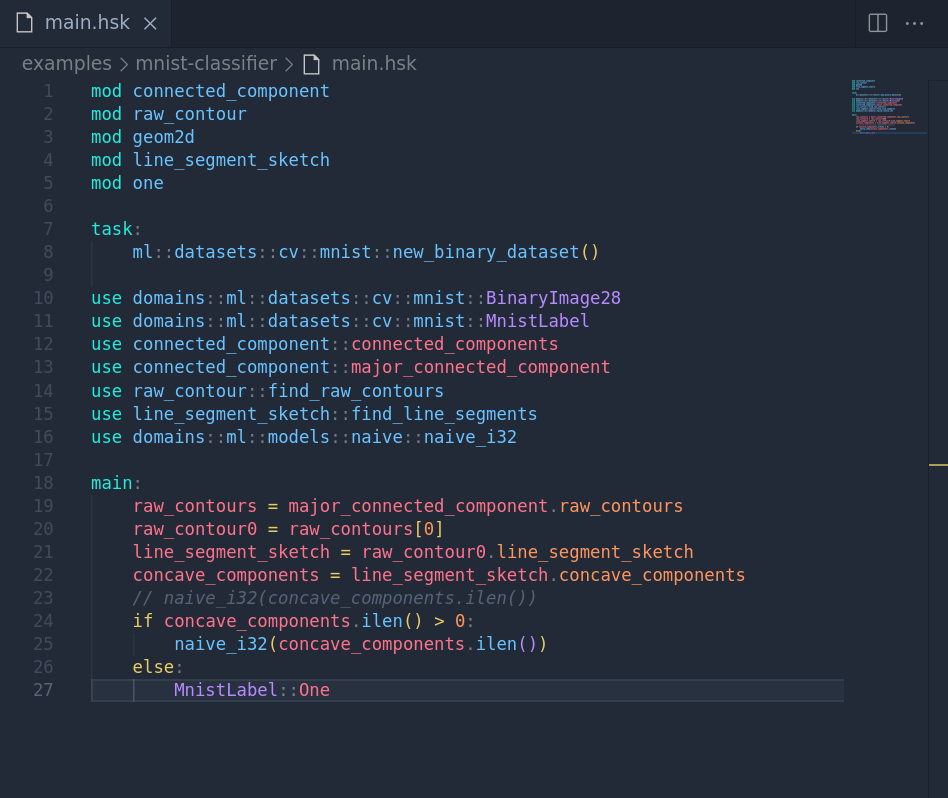
\includegraphics[width=\linewidth]{snapshots/old_syntax00}
\end{frame}

\begin{frame}
\frametitle{``Achievement''} Hand written code (without using any form of machine learning) for classifying hand-written digits (MNIST), 80\% accuracy, not much effort because of bugs

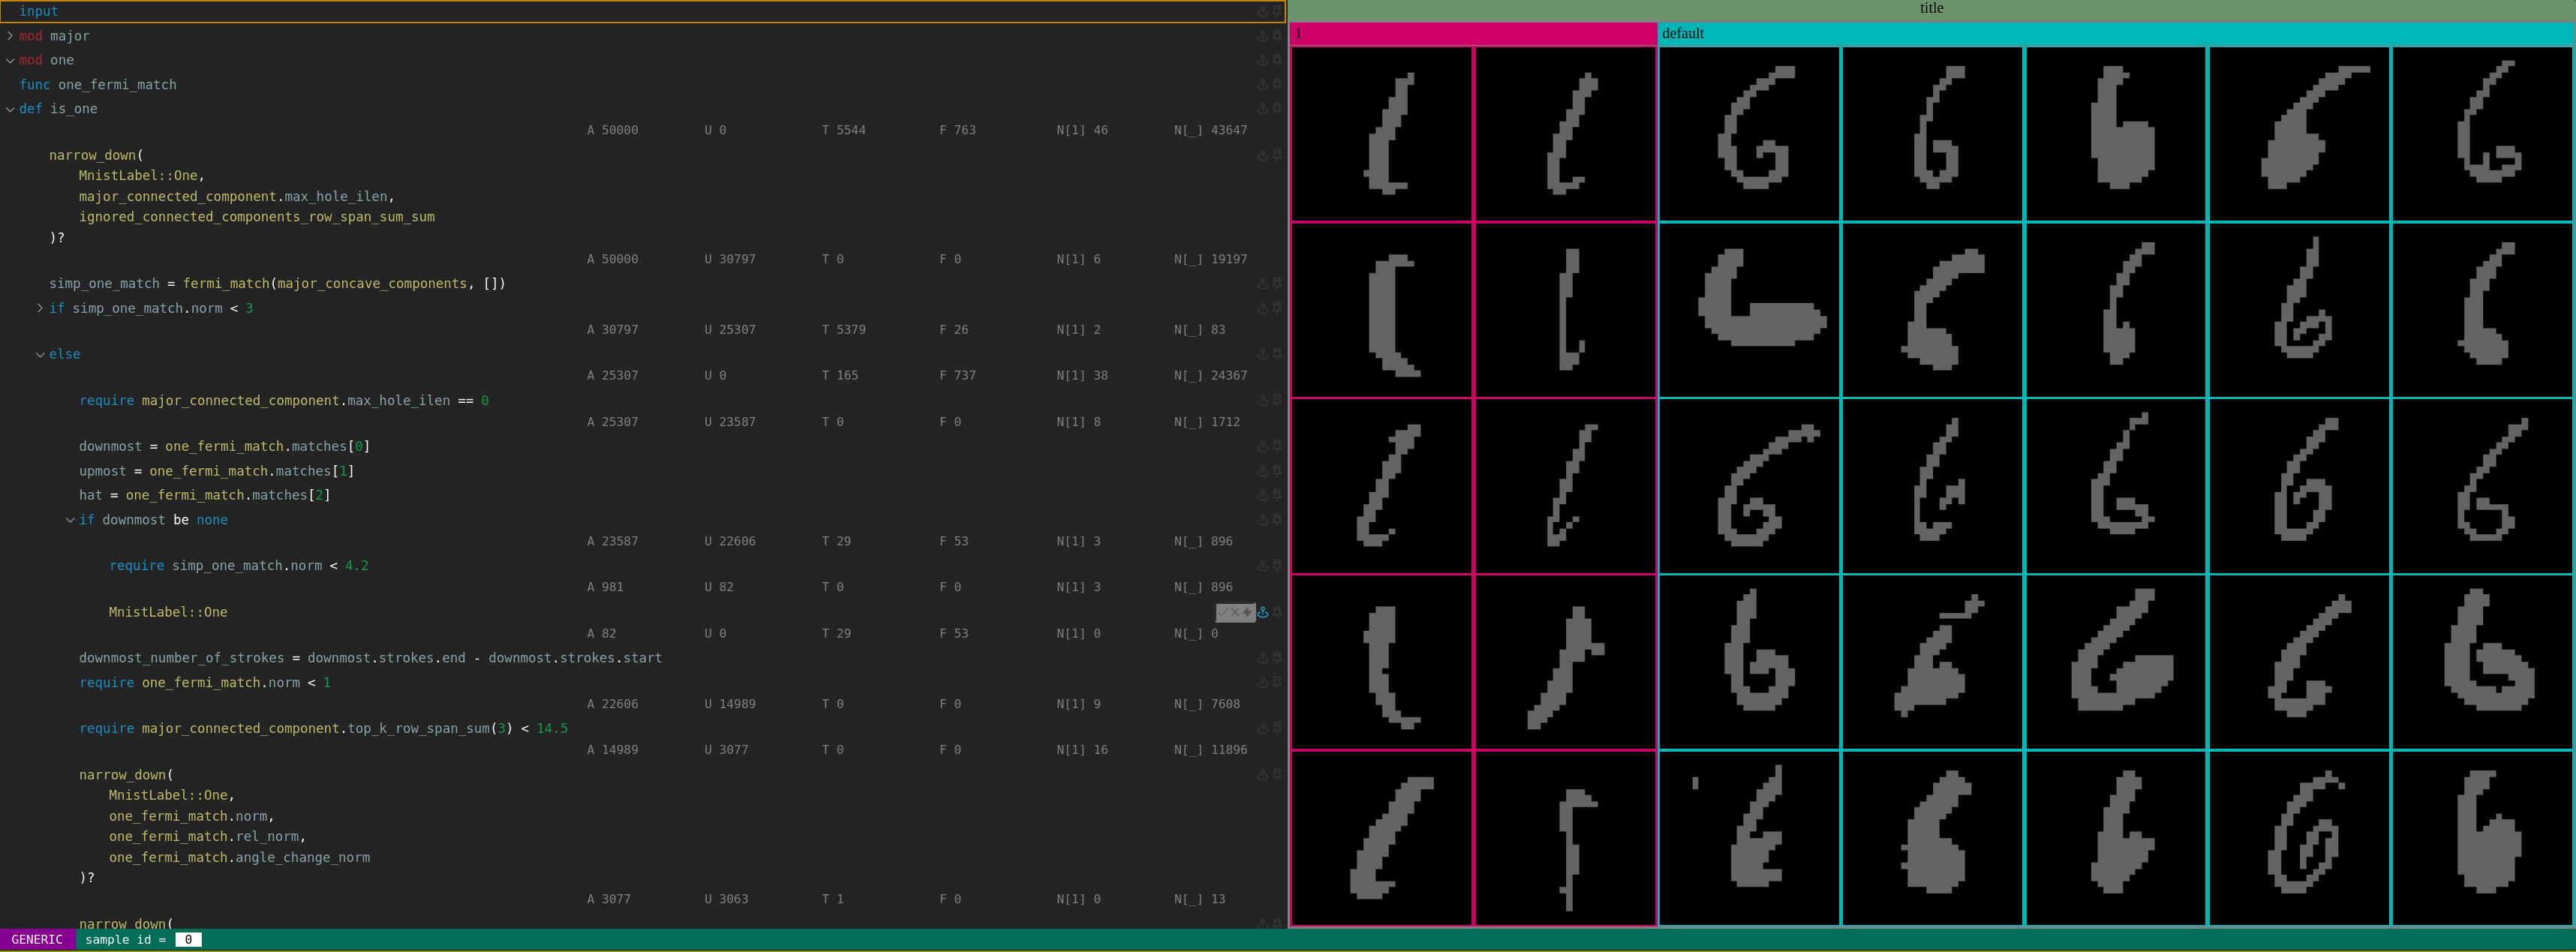
\includegraphics[width=\linewidth]{snapshots/mnist_debug_screenshot00.png}
\end{frame}

\begin{frame}
\frametitle{``Achievement''}

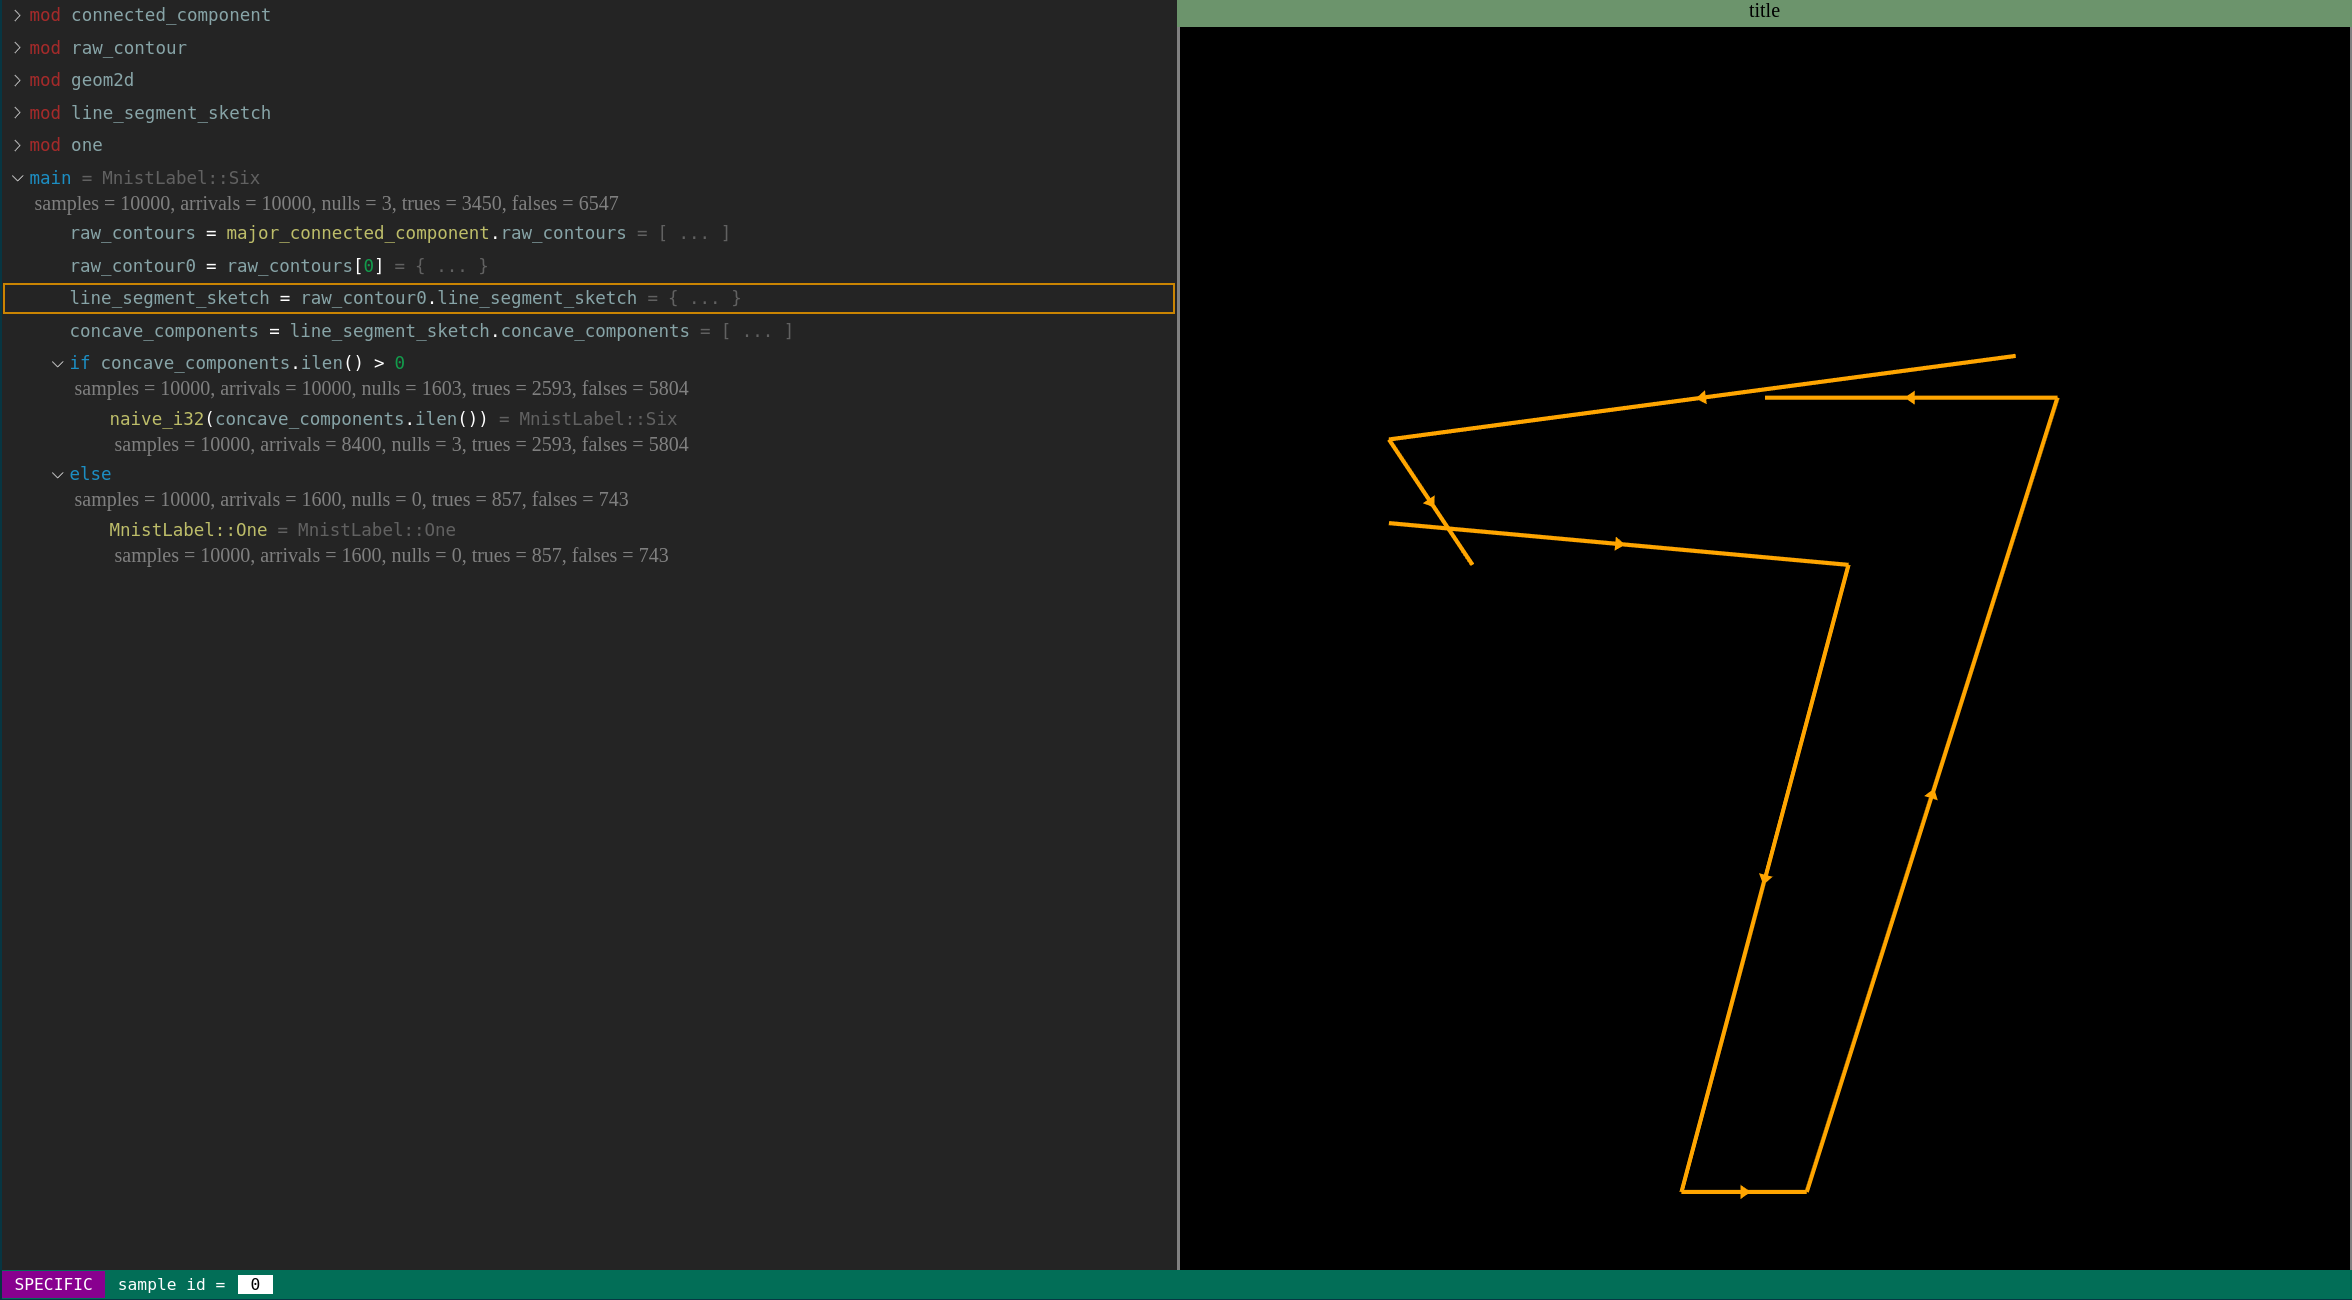
\includegraphics[width=\linewidth]{snapshots/mnist_debug_screenshot01.png}
\end{frame}

\begin{frame}
\frametitle{Status Quo}
\begin{itemize}
	\item In the progress towards a new powerful prototype, 116k Lines of well-structured code, 4k todos, 2k warnings.
	\item This version is very close to an industrial language, with
	\begin{itemize}
		\item package and module system.
		\item powerful type system (variance, generics, dependent type, traits).
		\item convenient symbol import (like Rust, better than Haskell and Lean).
		\item flexible type inference (like Rust).
		\item everything is optimized for incremental computation, refined caching based on region paths and type terms.
	\end{itemize}
	\item Syntax and semantics suffices for now, I'm working on debugging system, compilation etc.
\end{itemize}
\end{frame}

\begin{frame}
\frametitle{Near Future: Publish or Perish}
\begin{itemize}
	\item I'm rushing towards a new prototype
	\item In the following one or two years, I will use it for 
	\begin{itemize}
		\item new computer vision models that run faster on phones or IoT devices
		\item machine learning theories for image classification
	\end{itemize}
	\item it's about time to write papers
\end{itemize}
\end{frame}

\begin{frame}
\frametitle{Far Future: Keep Agile}
\begin{itemize}
	\item What I don't like is, run into stable version and then discover the features don't satisfy the needs.
	\item Agility: keep language unstable, test it for various tasks, and gradually adapt.
	\item 5-10 years from version 0.1, 15-20 years from version 1.0.
	\item Good enough to apply it for AI research within months.
	\item For production, transpile into C or Zig or even high level C++ or Rust.
\end{itemize}
\end{frame}



\section{Basic Designs}
\begin{frame}
\frametitle{Husky Merges Features of Modern Languages} 
\begin{itemize}
	\item its name `\textcolor{orange}{Husky}' comes from `\textcolor{orange}{H}a\textcolor{orange}{sk}ell' and `R\textcolor{orange}{us}t' and `p\textcolor{orange}{y}thon'
	\item its file extension `\textcolor{orange}{hsy}' comes from `\textcolor{orange}{hs}' (Haskell) `r\textcolor{orange}{s}' (Rust) and `p\textcolor{orange}{y}' (python)
	\item its package manager called `\textcolor{orange}{corgi}' is just like `cargo'
	\item its syntax is best described by `pythonic Rust' for runtime and Lean-like for comptime
	\item type system is influenced by Rust + Lean + ATS, with monad replaced by trait Unveil and effects, and new memory types are introduced
	\item it has a global computation graph like Haskell, or deep learning libraries
\end{itemize}
\end{frame}

\begin{frame}
\frametitle{Syntax}

Overall it's about system level and functional. No OOP but has methods and traits.

Looks like mojo because the design goals are similar.
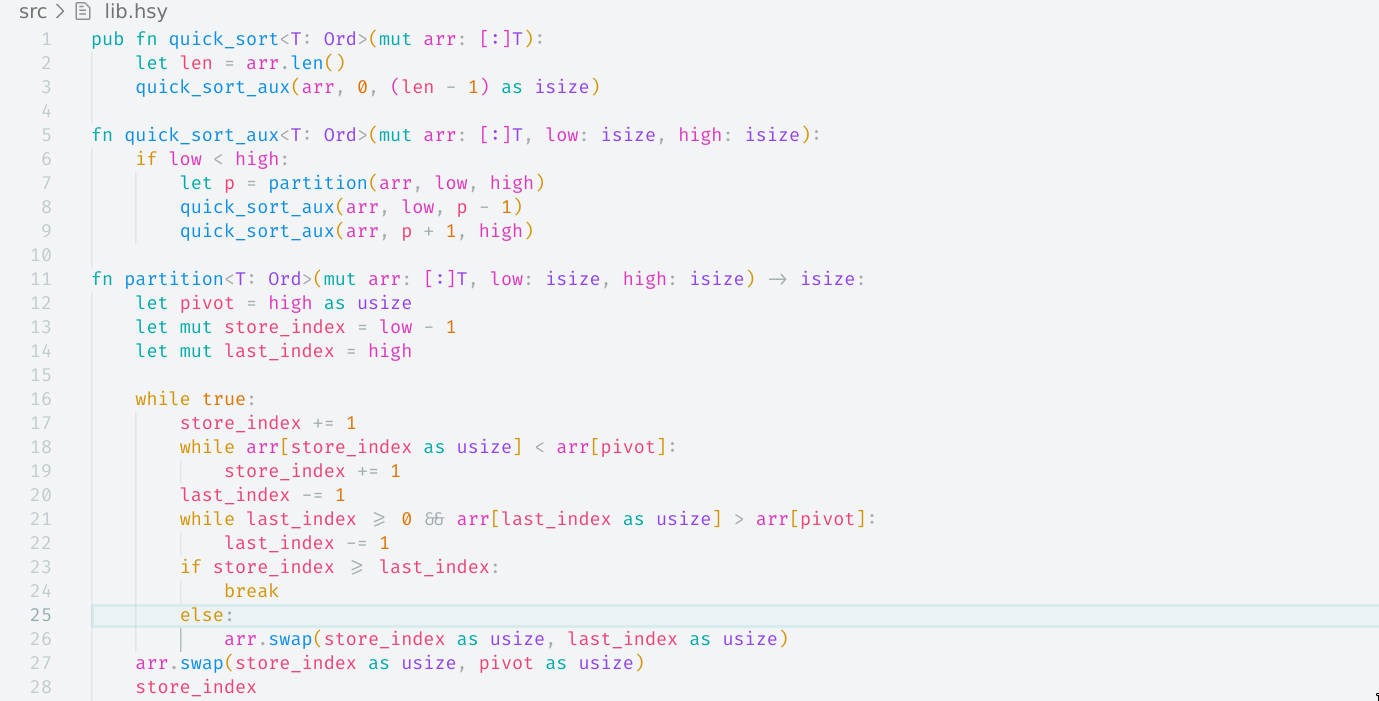
\includegraphics[width=\linewidth]{snapshots/husky_quick_sort.png}
\end{frame}

\begin{frame}
\frametitle{Syntax}

Symbol are introduced through `use', basically the same as Rust.

Package, crate, file layout are basically the same as Rust.
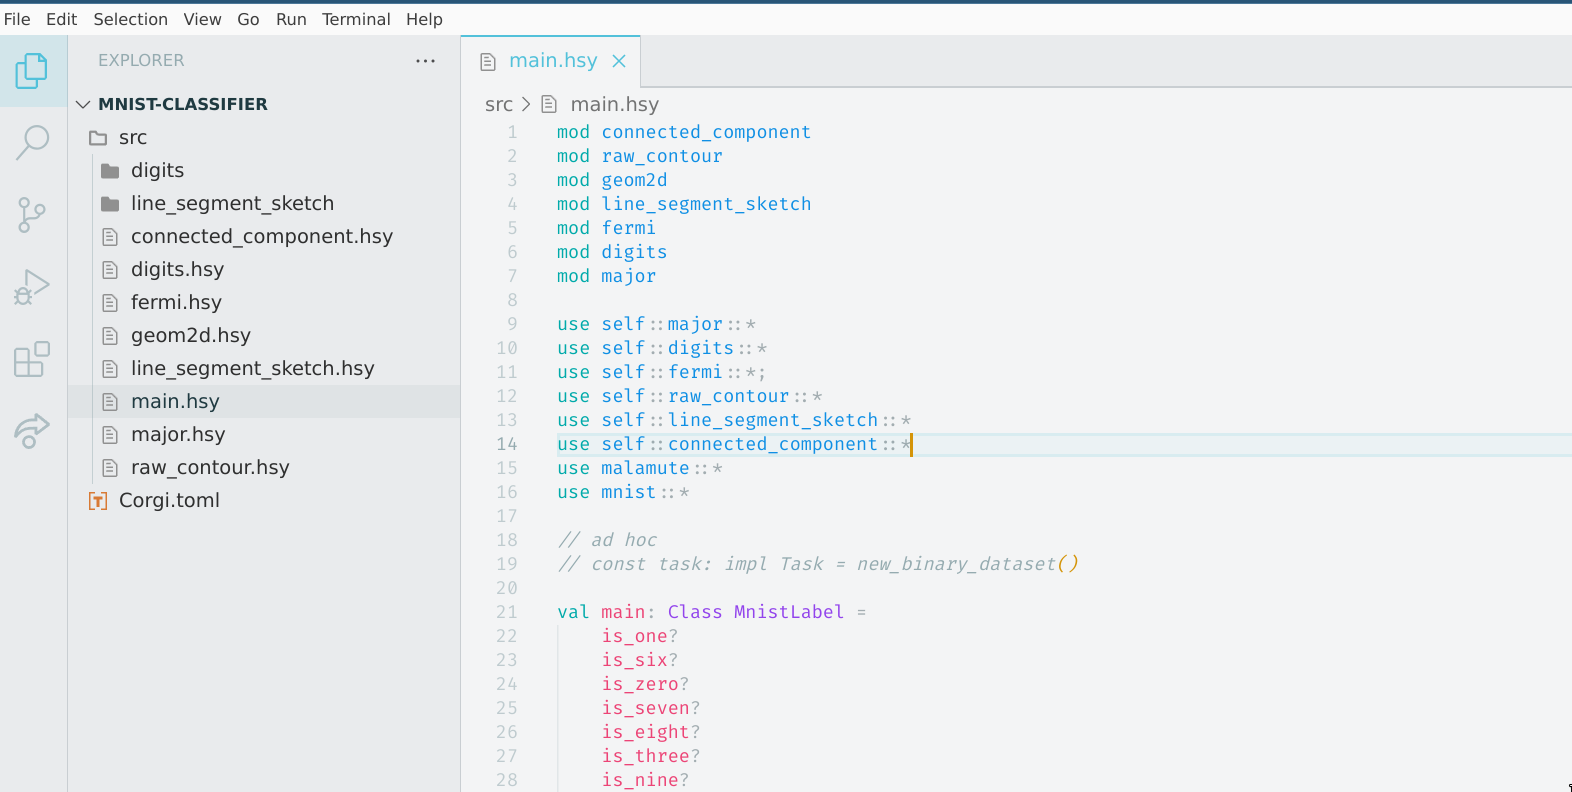
\includegraphics[width=\linewidth]{snapshots/husky_file_structure.png}
\end{frame}

\begin{frame}
\frametitle{Cargo is called Corgi}

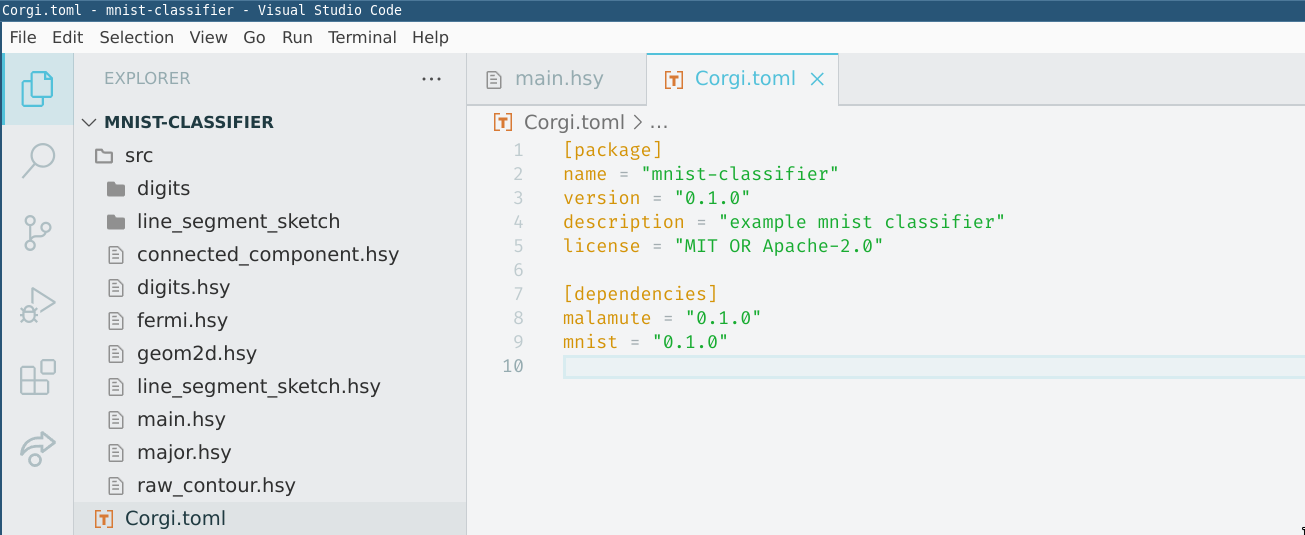
\includegraphics[width=\linewidth]{snapshots/husky_cargo_is_called_corgi.png}

In Rust, cargo configuration errors will cause compiler to panick.

But in Husky, corgi configuration errors are seen as syntax errors and there are customized toml parsers to make things as ergonomic as possible.
\end{frame}

\begin{frame}
\frametitle{Type Definition}

One can define
\begin{itemize}
	\item regular struct/structure
	\item tuple struct/structure
	\item unit struct/structure
	\item enum/inductive
	\item extern type
\end{itemize}

Here struct enum are for runtime values, and structure or inductive are for compile time (term level) values. The details are yet to be determined.
\end{frame}

\begin{frame}
\frametitle{Type Definition Examples}
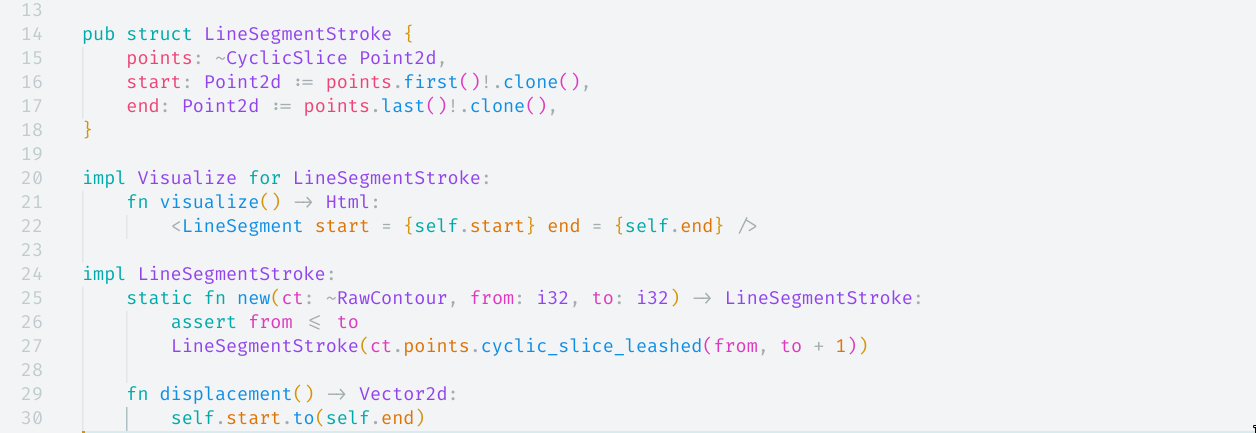
\includegraphics[width=\linewidth]{snapshots/husky_struct_definition.png}
\end{frame}

\begin{frame}
\frametitle{Type Definition Examples}
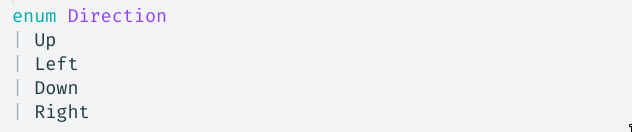
\includegraphics[width=\linewidth]{snapshots/husky_enum_definition.png}
\end{frame}


\begin{frame}
\frametitle{Algebraic data type realized just like Rust}
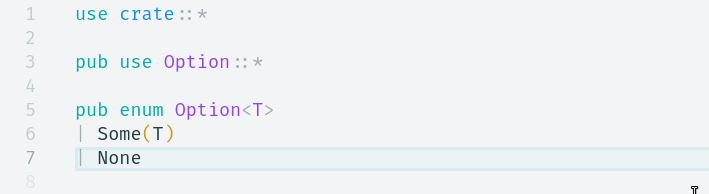
\includegraphics[width=\linewidth]{snapshots/husky_option_definition.png}
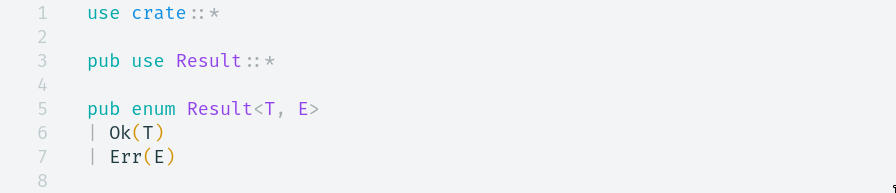
\includegraphics[width=\linewidth]{snapshots/husky_result_definition.png}
\end{frame}

\begin{frame}
\frametitle{Method}
I choose to allow self parameter to be omitted.

Use static for associated functions.
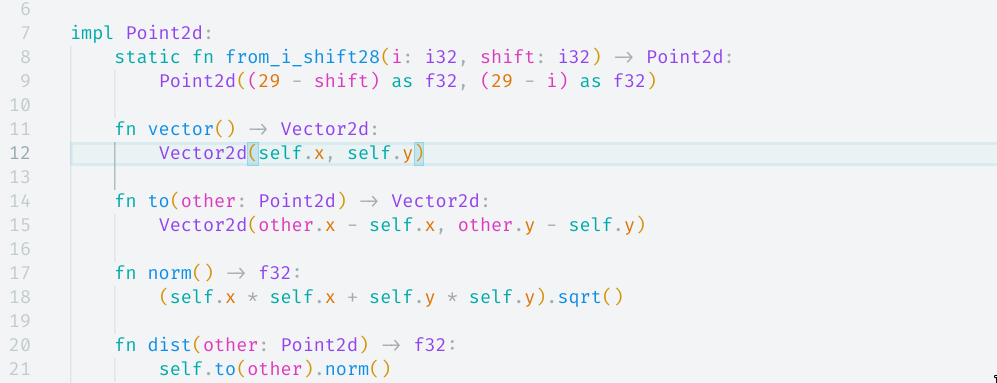
\includegraphics[width=\linewidth]{snapshots/husky_method.png}
\end{frame}

\begin{frame}
\frametitle{Trait}
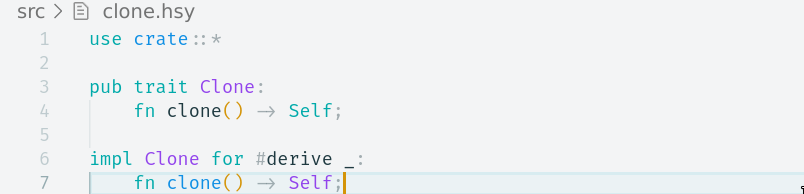
\includegraphics[width=\linewidth]{snapshots/husky_clone_derive_trait_side.png}
\end{frame}

\begin{frame}
\frametitle{Derive Trait}
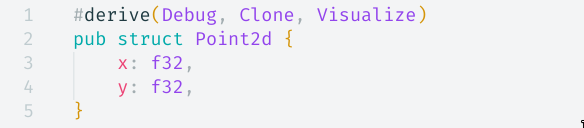
\includegraphics[width=\linewidth]{snapshots/husky_clone_derive_example.png}

In the above $\#derive$ is not a macro, but an attribute, serving as a marker. In the original trait definition, there could be a implementation of the trait for all marked types, with a generic representation of a general type, as inpired by Haskell's macro system. Details are to be determined.
\end{frame}

\begin{frame}
\frametitle{Macro}
There is no macro in husky.

Macro = undefined behavior of compilers

Husky stays as a research language in foreseeable future, so there is no pressure to be popular.
\end{frame}

\begin{frame}
\frametitle{Type System}
Design goals:
\begin{itemize}
	\item Easy as python to write
	\item Safe as ATS, no undefined behaviors,
	\item Zero-Cost and practical as Rust and C++
\end{itemize}

Layers of type system (necessarily complicated for efficiency, expressiveness):
\begin{itemize}
	\item Declarative Term. Easily read from syntax tree, but can be ambiguous Used in the first step for type signature inference.
	\item Ethereal Term. Target efficient caching.
	\item Fluffy Term. Target borrow checking. Not stored globally.
	\item Hir Type. Close to Rust. Unnecessary terms are thrown away (phantom arguments, univalent values, etc)
\end{itemize}
\end{frame}

\begin{frame}
\frametitle{Declarative Term for Type Signature Inference}
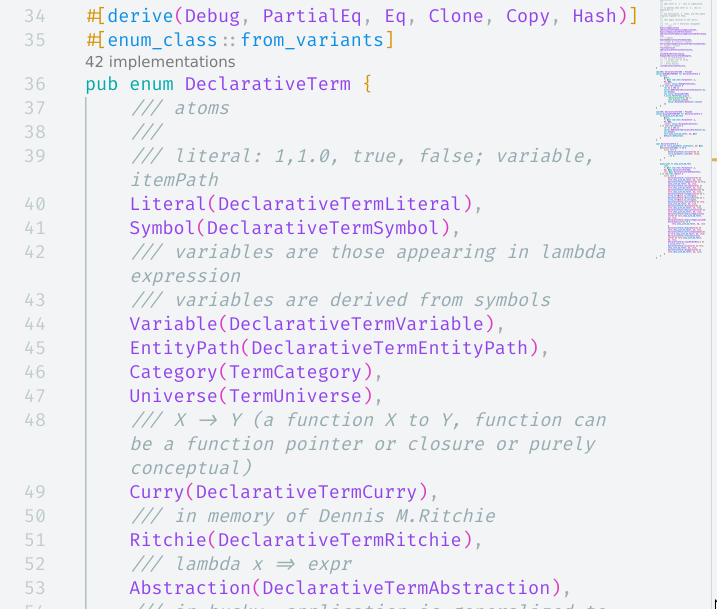
\includegraphics[width=\linewidth]{snapshots/husky_declarative_term.png}
\end{frame}

\begin{frame}
\frametitle{Ethereal Term for Caching}
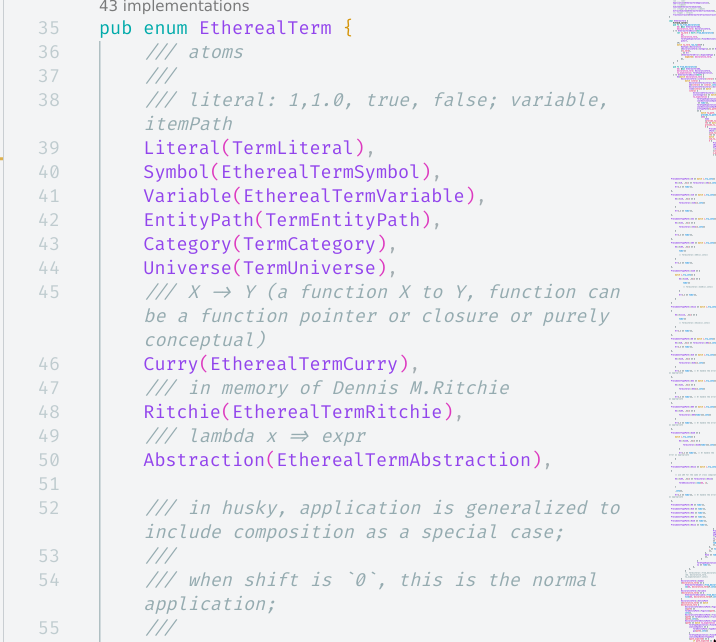
\includegraphics[width=\linewidth]{snapshots/husky_ethereal_term.png}
\end{frame}

\begin{frame}
\frametitle{Fluffy Term for Borrow Checking}
Fluffy terms are not saved globally because cache hits are hard.
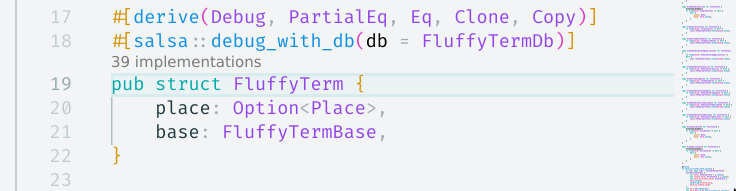
\includegraphics[width=\linewidth]{snapshots/husky_fluffy_term.png}
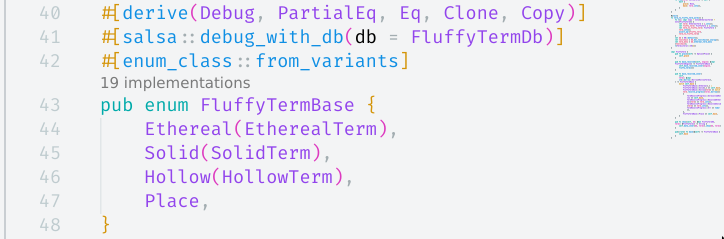
\includegraphics[width=\linewidth]{snapshots/husky_fluffy_term2.png}
\end{frame}

\begin{frame}
\frametitle{Hir Type for Compilation}
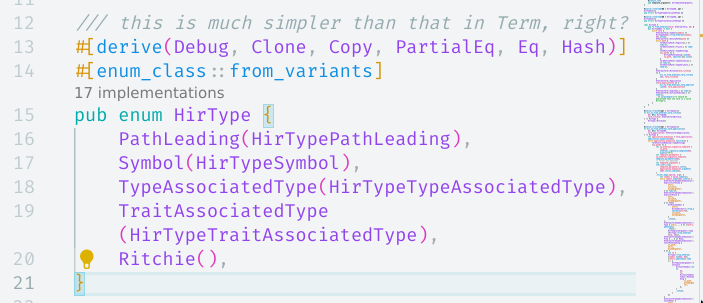
\includegraphics[width=\linewidth]{snapshots/husky_hir_ty.png}
\end{frame}

\begin{frame}
\frametitle{Variance}
Basically the same as Rust. For extern generic type, variance can be explicitly declared,
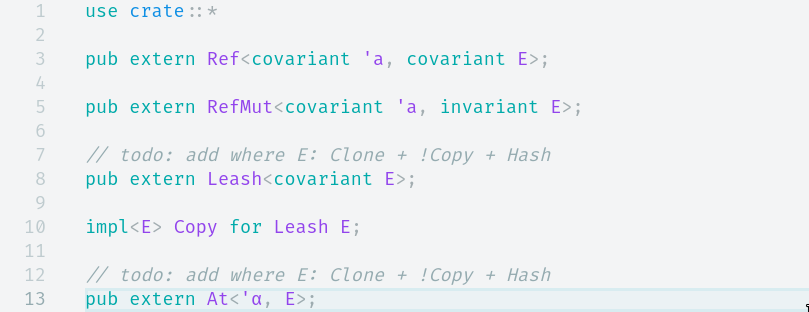
\includegraphics[width=\linewidth]{snapshots/husky_variance.png}

Of course, having variance makes type inference more complicated.
\end{frame}

\begin{frame}
\frametitle{Memory Types}
Husky has more memory types than Rust
\begin{itemize}
	\item Leash type.
	\item Pure Access.
	\item At type.
\end{itemize}
\end{frame}

\begin{frame}
\frametitle{Leash type}
Denoted by $\sim$. This symbol was used for Box in early Rust.

Leash type is for access values stored in global database. Similar to salsa. However, Leash type is like a universal interface, one can easily customize its implementation for specific tasks. One can implement it as static reference or garbage collected reference.
\end{frame}

\begin{frame}
\frametitle{Leash In Action}
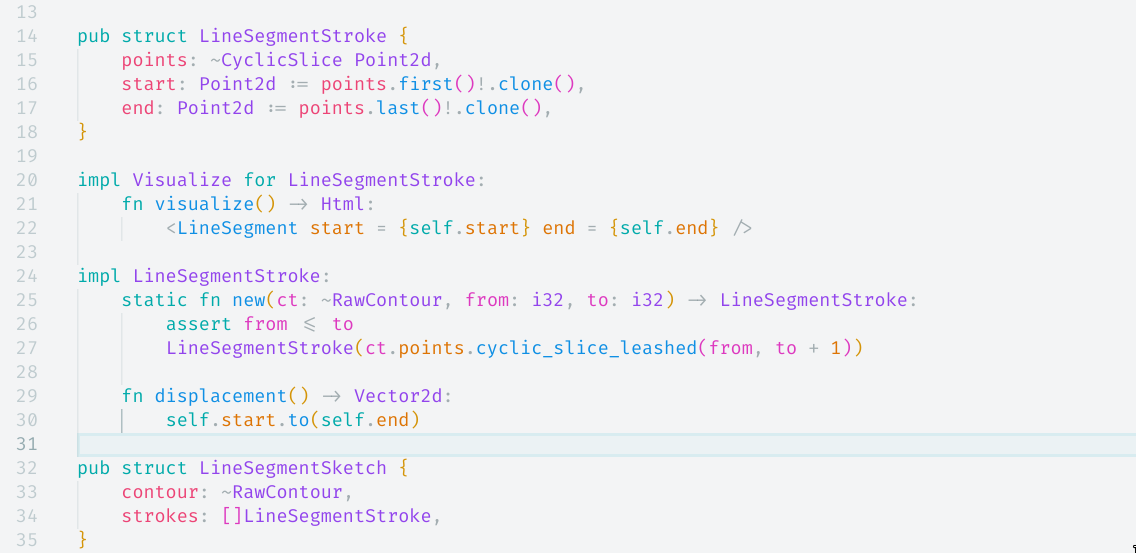
\includegraphics[width=\linewidth]{snapshots/husky_leash_in_action.png}
\end{frame}

\begin{frame}
\frametitle{Leash Can Have Memoized Field}
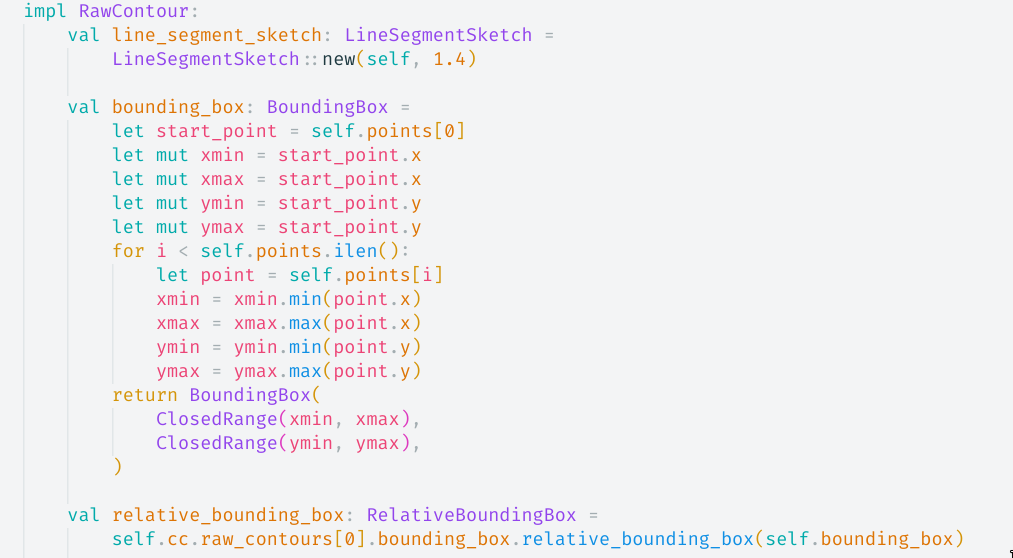
\includegraphics[width=\linewidth]{snapshots/husky_memoized_field.png}
\end{frame}

\begin{frame}
\frametitle{Pure Access}

It's a type alias or functor, \husky{PureAccess T} for a runtime type \husky{T} is equal to
\begin{itemize}
	\item itself, if \husky{T} is copyable
	\item a reference to \husky{T}, otherwise
\end{itemize}

A function argument type is pure access by default.

In Rust, using get method of HashMap requires a reference to the key, even if the key is copyable. This problem is solved in Husky through pure access.
\end{frame}

\begin{frame}
\frametitle{Place and At Type}
Rust introduces the concept of \textcolor{orange}{lifetime}, so does Husky, but Husky also introduces \textcolor{orange}{place}. 

{\color{gray}Afterall, time and space is the same thing according to Einstein.}

Special thanks to Bjarne Stroustrup. This is influenced by \cpp{const} lvalue and rvalue in C++.
\end{frame}

\begin{frame}
\frametitle{Place and At Type: Rust Side Definition}

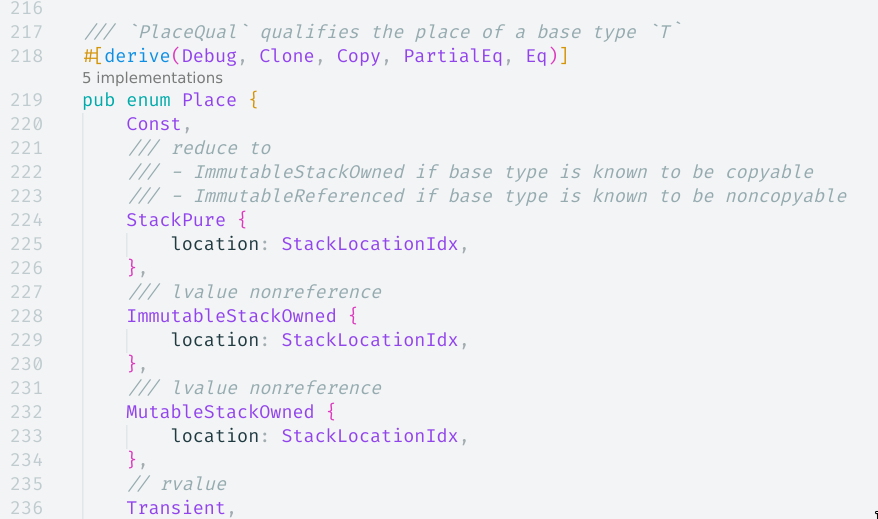
\includegraphics[width=\linewidth]{snapshots/husky_place_defn00.png}
\end{frame}

\begin{frame}
\frametitle{Place and At Type: Rust Side Definition Continued}

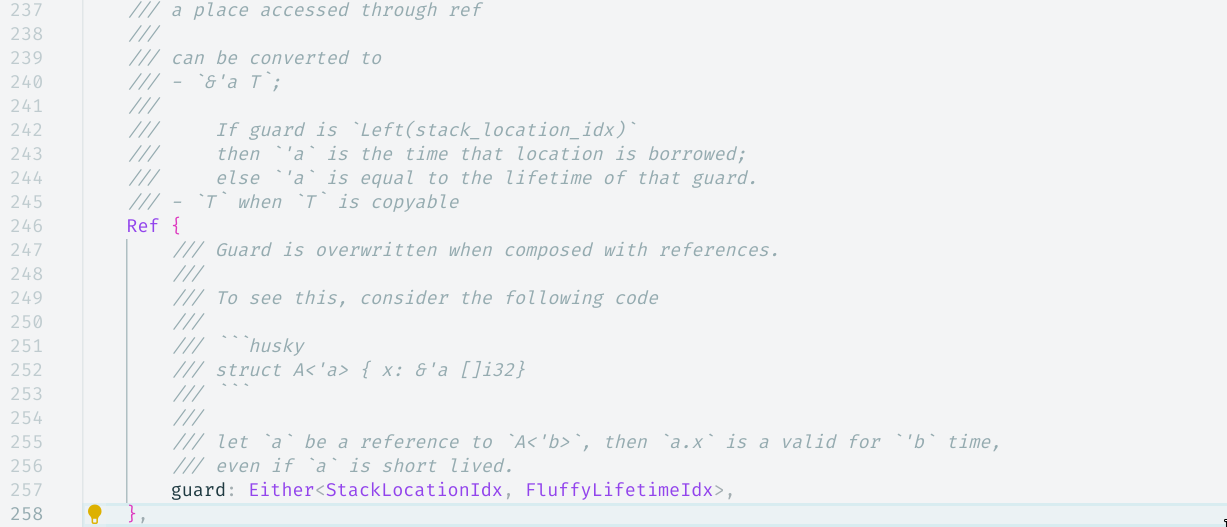
\includegraphics[width=\linewidth]{snapshots/husky_place_defn01.png}
\end{frame}

\begin{frame}
\frametitle{Place and At Type: Rust Side Definition Continued}

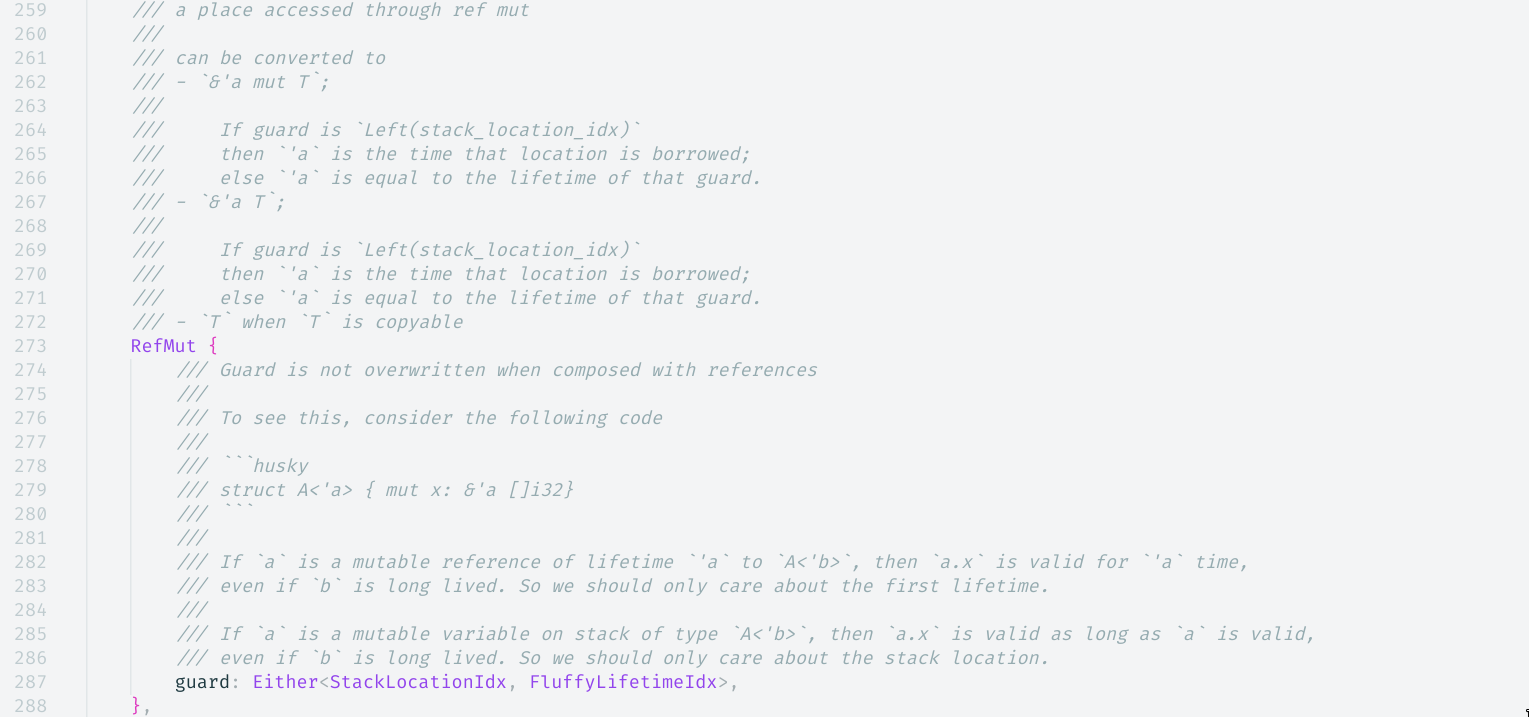
\includegraphics[width=\linewidth]{snapshots/husky_place_defn02.png}
\end{frame}

\begin{frame}
\frametitle{Place and At Type: Rust Side Definition Continued}

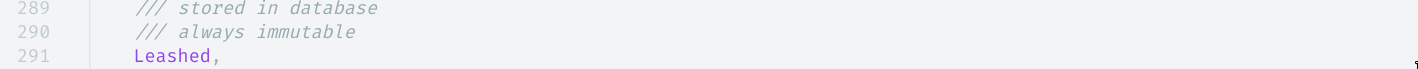
\includegraphics[width=\linewidth]{snapshots/husky_place_defn03.png}

This list is not exhaustive.

Place can include device information such as cpu/gpu.

\husky{At} Type is simply a type together with a place. Written as @'$\alpha$ \husky{t} where '$\alpha$ is a label representing a place and \husky{t} a type. It's customary to use Latin letter labels for lifetime and greek letter labels for place.
\begin{itemize}
	\item it can be coerced implicitly from/to other types like leash, reference, mutable reference, etc, depending on specific place value.
	\item place can be generic, thus no need for \rust{last_mut} like in Rust.
\end{itemize}
\end{frame}

\begin{frame}
\frametitle{Generic Place}
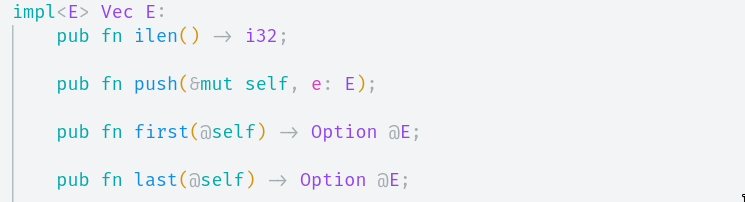
\includegraphics[width=\linewidth]{snapshots/husky_generic_place.png}

In the above, the method \husky{first} and \husky{last} has an implicit place template parameter. There is no need to define \husky{first_mut} and \husky{last_mut} as in Rust.
\end{frame}

\begin{frame}
\frametitle{Place and At Type}
At type is central to husky's type inference system. With it, one can write like python but the compiler will understand at a system level.
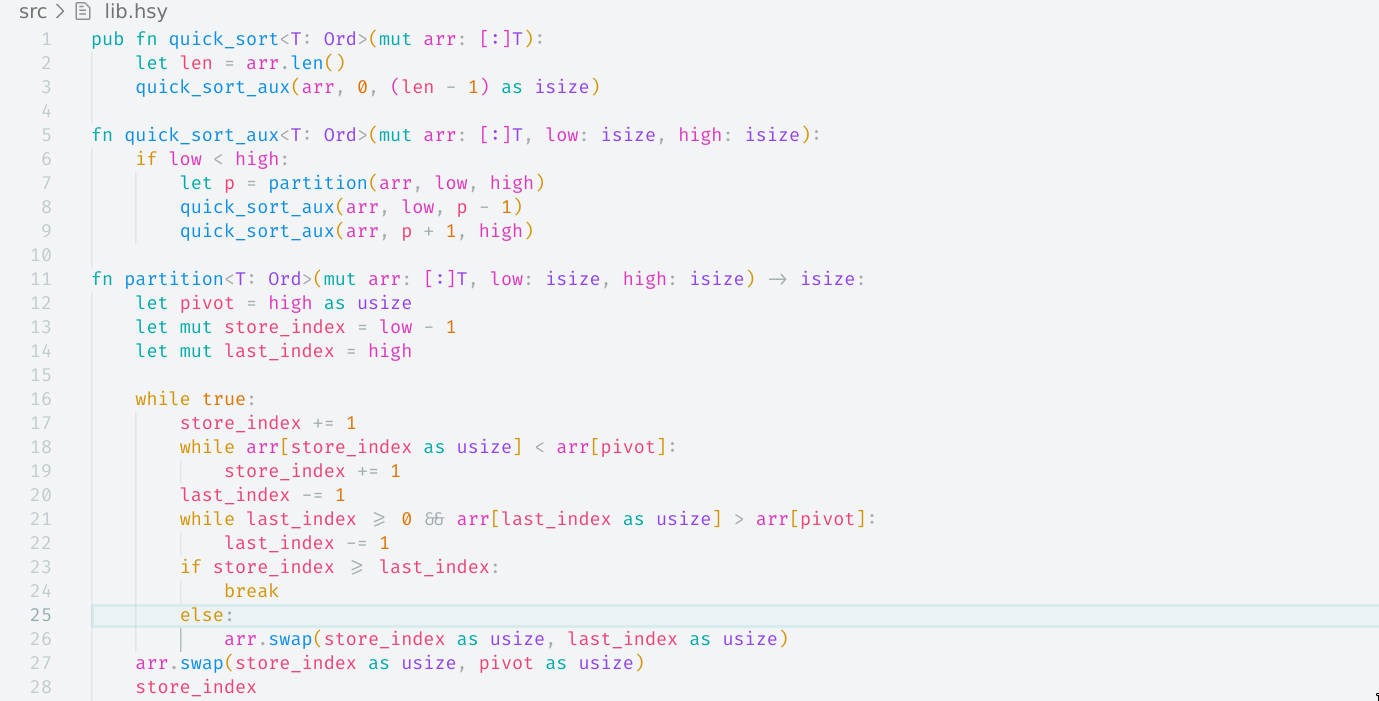
\includegraphics[width=\linewidth]{snapshots/husky_quick_sort.png}
\end{frame}

\begin{frame}
\frametitle{Place and At Type}
An expression like \rust{a.x} in Rust can be only understood as move or copy.

But Husky interprets the type of \husky{a.x} as a at type, with its place derived from that of \husky{a}.
\end{frame}

\begin{frame}
\frametitle{Borrow Checking in Rust}
In Rust, lifetime is analyzed ``statically''. 

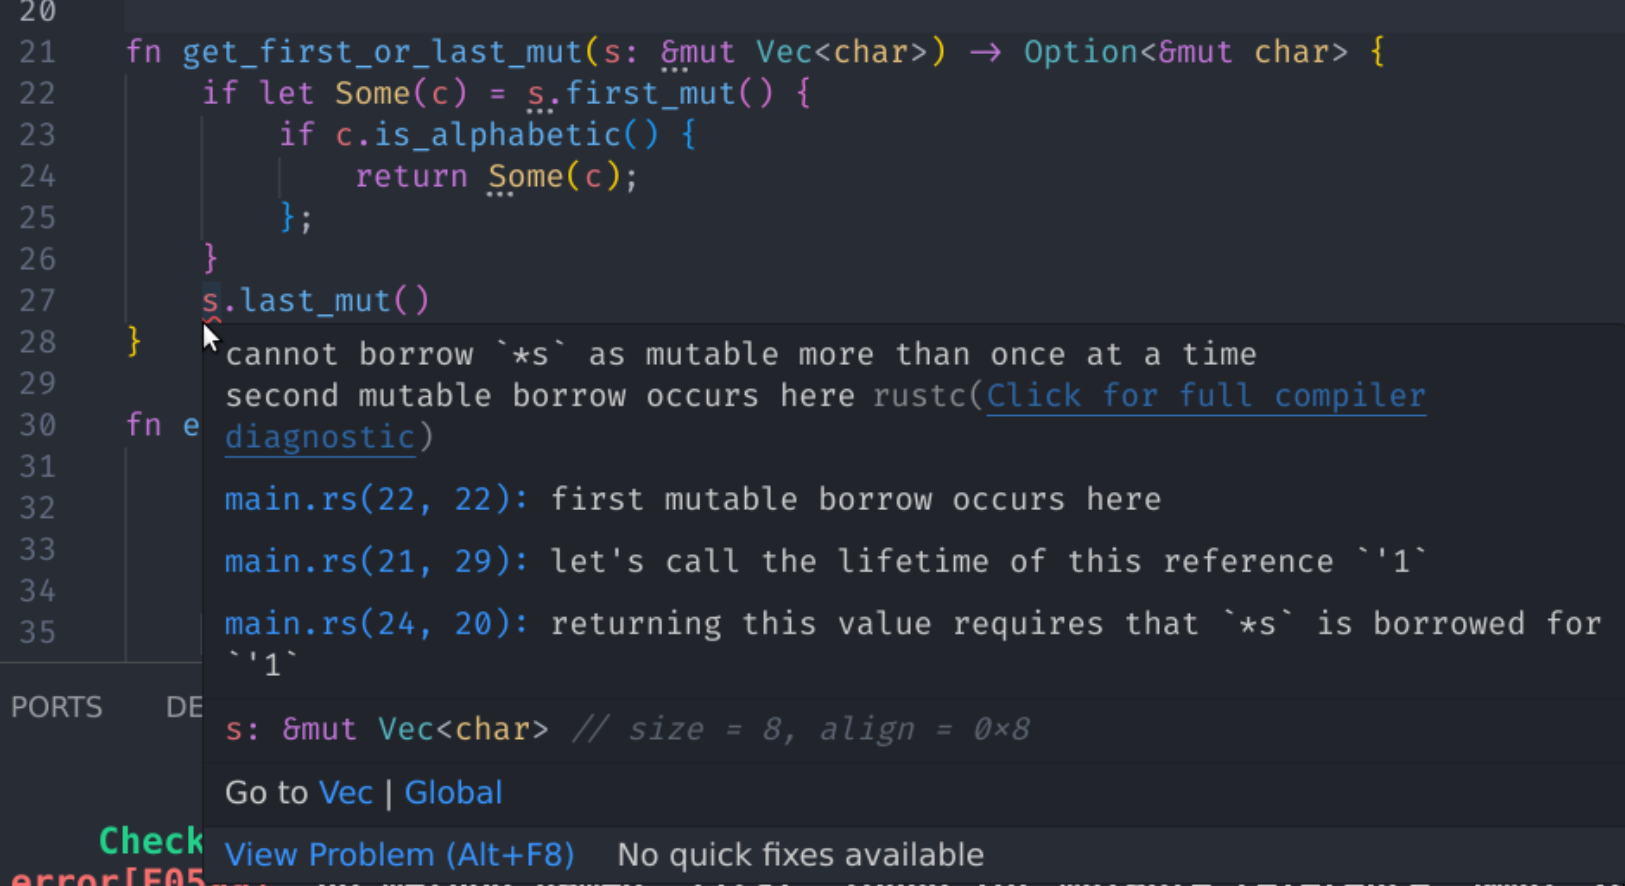
\includegraphics[width=\linewidth]{snapshots/get_first_or_last_mut.png}
\end{frame}

\begin{frame}
\frametitle{Borrow Checking in Husky}
In Husky I've invented a `dynamic' way of checking, enabling more safe code to pass borrow checking and maybe also more efficient.

{\color{gray}However, I have seen a paper from Germany that looks like doing similar things.}

In Husky, just collect all lifetime constraints and simply run a `symbolic simulation' to detect lifetime conflicts, with special handles for branches and loops.
\end{frame}

\begin{frame}
\frametitle{Monad}

Monad is fun and useful.
\begin{itemize}
	\item Functional way of defining Monad is too painful.
	\item Rust way of adopting Monad is much clearer, but can't handle effect and a little cumbersome to implement
	\item Husky simplifies Rust's way and combine with effectual system
\end{itemize}

\end{frame}

\begin{frame}
\frametitle{Monad through Effect and Unveil}
In Rust,
\begin{itemize}
	\item effectual monads like IO are not introduced.
	\item branching monads like Result and Option, however, are realized through traits \mintinline{Rust}{std::ops::Try} and \mintinline{Rust}{std::ops::FromResidual}
	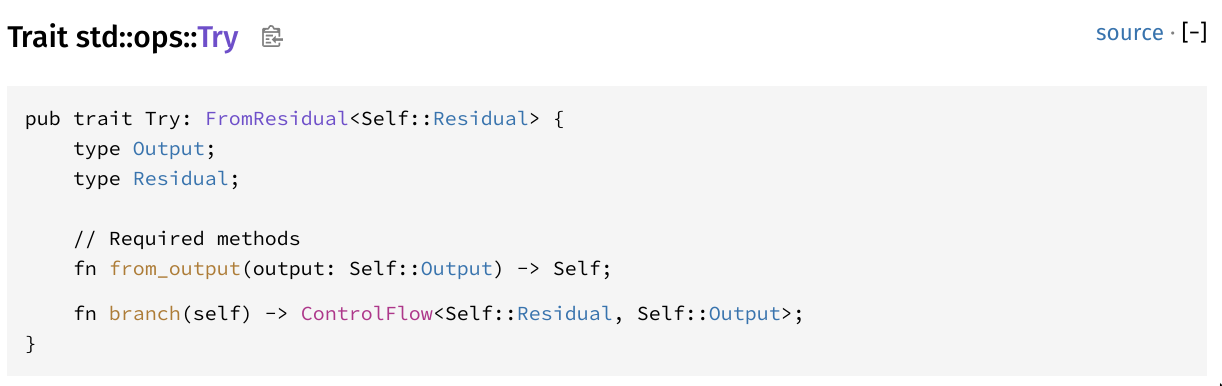
\includegraphics[width=\linewidth]{snapshots/rust_std_ops_try.png}
\end{itemize}
\end{frame}

\begin{frame}
\frametitle{Monad in Rust}
In Rust,
\begin{itemize}
	\item effectual monads like IO are not introduced.
	\item branching monads like Result and Option, however, are realized through traits \mintinline{Rust}{std::ops::Try} and \mintinline{Rust}{std::ops::FromResidual}
	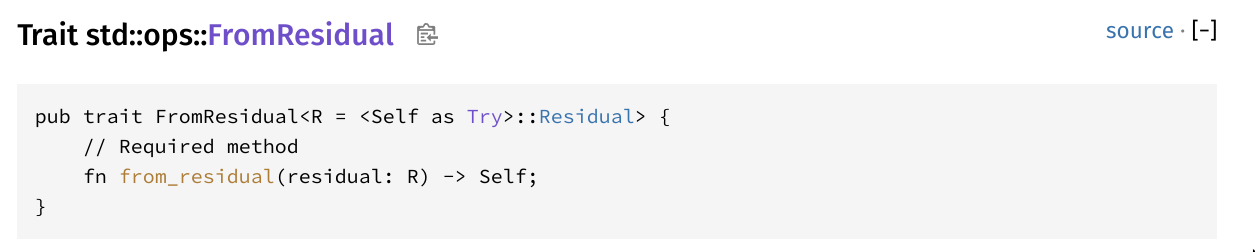
\includegraphics[width=\linewidth]{snapshots/rust_std_ops_from_residual.png} 
\end{itemize}
\end{frame}

\begin{frame}
\frametitle{Monad in Husky}
 In Husky, effects will be handled through attributes on functions and branching is realized through a single trait \mintinline{Rust}{core::ops::Unveil}.

Type \rust{A} implements \mintinline{Rust}{core::ops::Unveil} \rust{B} means that if a function return \rust{A}, then an expression of type \rust{B} in its body can be unveiled.

 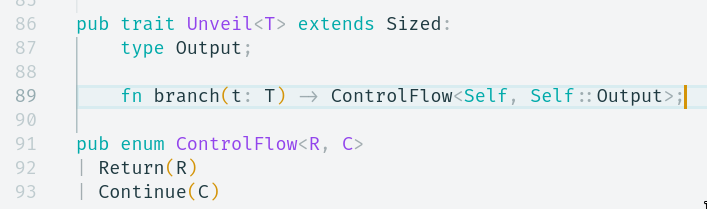
\includegraphics[width=\linewidth]{snapshots/husky_core_ops_unveil.png}
\end{frame}

\begin{frame}
\frametitle{Monad Implementation}
\mintinline{Rust}{Result} monad in Husky, from standard library (not complete yet, trait constraints are missing)

 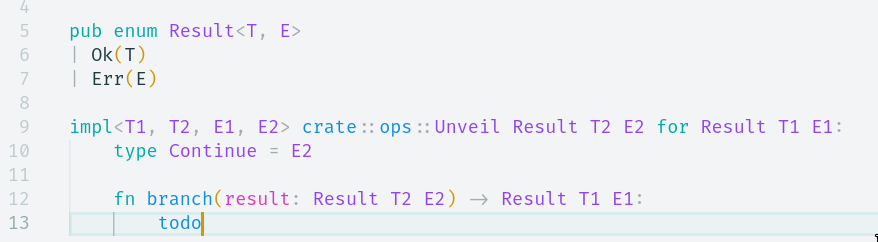
\includegraphics[width=\linewidth]{snapshots/husky_impl_unveil_for_result.png}
\end{frame}

\begin{frame}
\frametitle{Monad Implementation}
\mintinline{Rust}{Class} monad in Husky for classification tasks in machine learning, from custom package

 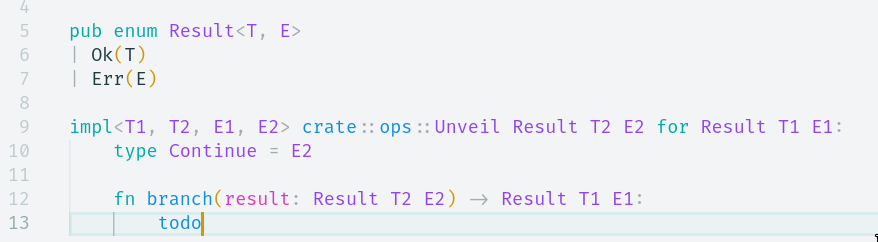
\includegraphics[width=\linewidth]{snapshots/husky_impl_unveil_for_result.png}
\end{frame}


\begin{frame}
\frametitle{Monad in Action}

In Husky, we use the same \rust{?} operator like in Rust to express branching

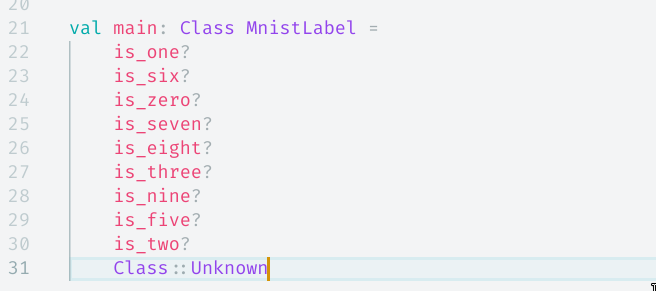
\includegraphics[width=\linewidth]{snapshots/husky_mnist_classifier_main.png}
\end{frame}

\begin{frame}
\frametitle{Monad in Action}
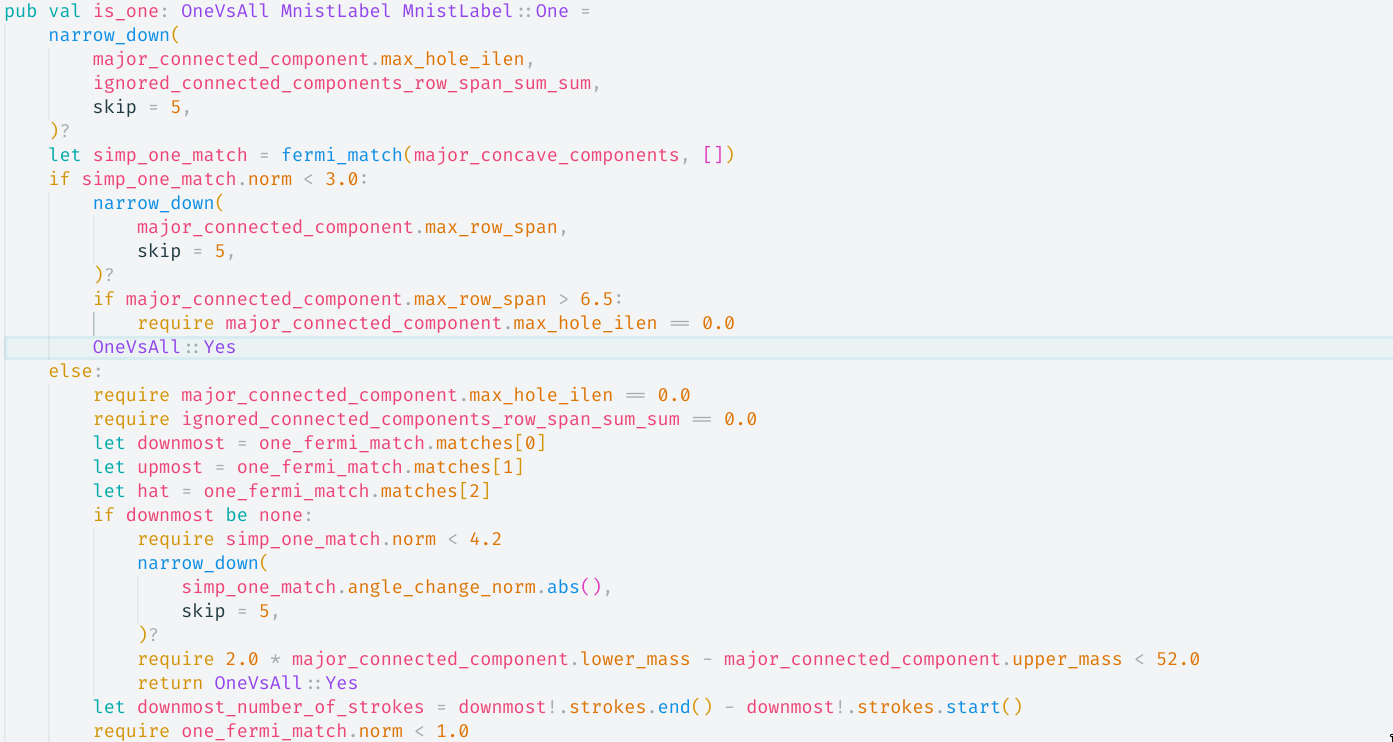
\includegraphics[width=\linewidth]{snapshots/husky_mnist_classifier_is_one.png}
\end{frame}

\begin{frame}
\frametitle{More Advanced Type System}
\begin{itemize}
	\item Dependent type. The type of generic function is actually dependent type. This is needed to have type safe AI models.
	\item Theorem proving. There are plans for them. Lean proves that there is no need for separate language like Coq and Ocaml. ATS proves that system level programming can be combined with theorem proving. Husky is going to continue this line of work.
\end{itemize}
\end{frame}

\begin{frame}
\frametitle{Task System}
In Husky one can fully customize compilation, runtime, debugging and visualization.

A task is an instance of a type that satisfies \rust{IsTask} trait. This trait exists both in Rust and in Husky.

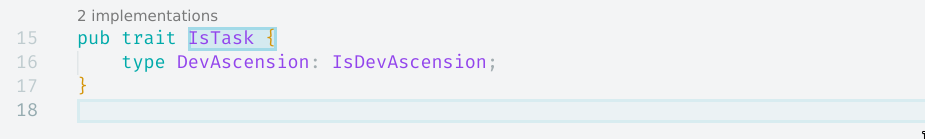
\includegraphics[width=\linewidth]{snapshots/husky_is_task_trait.png}
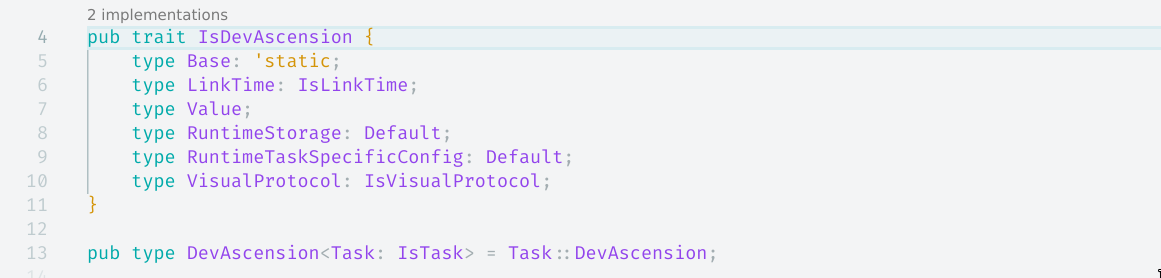
\includegraphics[width=\linewidth]{snapshots/husky_is_dev_ascension_trait.png}
\end{frame}

\begin{frame}
\frametitle{Task Example}
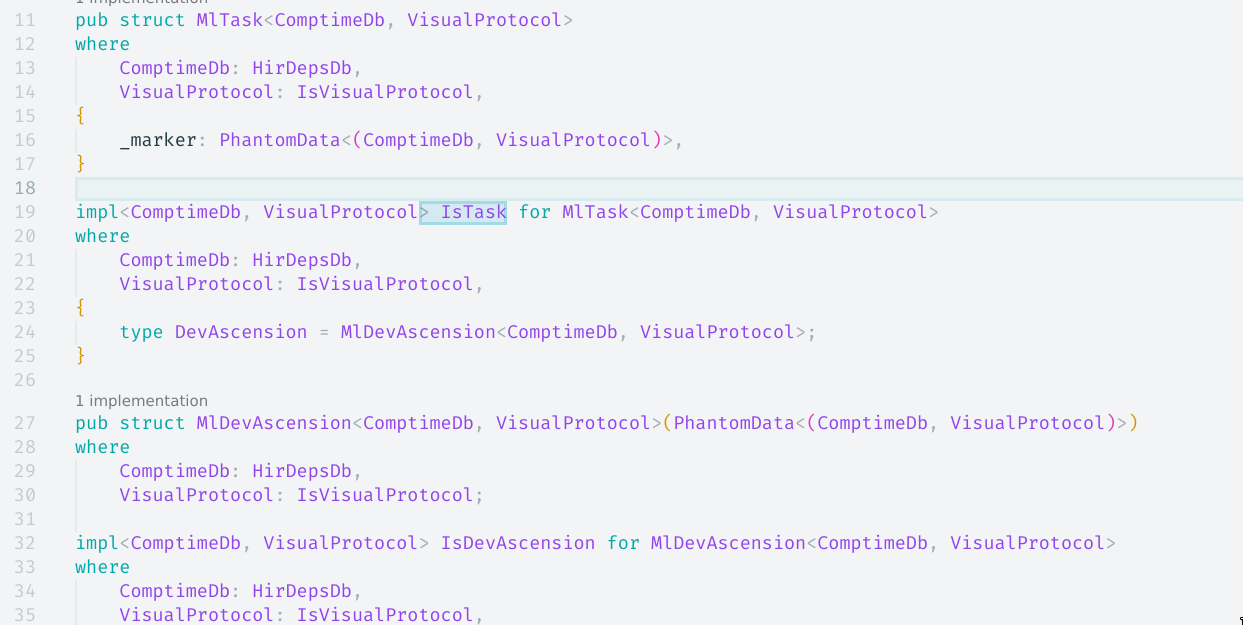
\includegraphics[width=\linewidth]{snapshots/husky_is_task_example_implementation.png}
\end{frame}

\begin{frame}
\frametitle{Task Specification}
Task (type and instance) is specified in the root of an executable crate by a zero argument function named task.

For libraries, one might need to specify some traits the task type needs to satisfy.
\end{frame}

\begin{frame}
\frametitle{Why So Much Trouble?}
Different tasks require different strategies for compilation, evaluation, debugging. Husky will have very good development experience thanks to this.

\begin{itemize}
	\item Mixture of interpretation and compilation saves incremental compilation speed by minimizing dependency tree.
	\item Certain task can have a top level computation graph, and husky support incremental evaluation so that values are automatically kept up to date with little computation. Say goodbye to jupyter notebook
	\item Support for custom memory allocation and reference strategies.
\end{itemize}
\end{frame}

\begin{frame}
\frametitle{Husky Stands on Giants' Shoulders}

The complicated design of Husky is built upon amazing previous works.
\end{frame}

\section{Ascension Paradigm}

\begin{frame}
\frametitle{Functional Programming vs Procedural Programming}
\begin{itemize}
	\item Functional Programming
	\begin{itemize}
		\item Close to logic
		\item Easy to do high level optimization

		\textcolor{gray}{incremental computation, laziness, etc.}
		\item Hard to do low level optimization
	\end{itemize}
	\item Procedural Programming
	\begin{itemize}
		\item Close to hardware
		\item Easy to do low level optimization
		\item Hard to do high level optimization

		\textcolor{gray}{mutable state, loops, small vectors}
	\end{itemize}
	\item Compilers are not AGIs. How to get the best of both worlds?
\end{itemize}
\end{frame}

\begin{frame}
\frametitle{Combining Functional and Procedural Programming}
Past efforts are
\begin{itemize}
	\item Rust salsa. incremental computation. macro heavy.
	\item Every deep learning framework.
	\item Reactive programming for UI programming. Svelte, Elm.
\end{itemize}

In Husky, ascension paradigm is a general way of combining functional and procedural programming. It can express salsa and svelte as special cases.

{
\color{gray}
salsa and deep learning frameworks are just computation graphs, but reactive programming is something more. In Husky's perspective, the latter requires ascension, the former does not.}
\end{frame}

\begin{frame}
\frametitle{Mathematical Definition of Computation Graph}
Let $G$ be a directed graph with vertices $V$ and edges $E$.

For any $v\in V$, assign a variable $x_v$ of type $t_v$.

For each source vertex $v$, $x_v$ is interpreted as input.

For each nonsource vertex $v$ with $n$ incoming vertices $v_1,\cdots,v_n$, we add a relationship

$$x_v=f_v(x_{v_1},\cdots,x_{v_n})$$

for a function $f_v$ of type $t_{v_1}\to\cdots\to t_{v_n}\to t_v$.
\end{frame}

\begin{frame}
\frametitle{Trivial Example of Computation Graph}
\begin{center}
\begin{tikzpicture}
  % Nodes
  \node[circle, draw, minimum size=1.5cm] (X) at (0,2) {x};
  \node[circle, draw, minimum size=1.5cm] (Y) at (0,0) {y};
  \node[circle, draw, minimum size=1.5cm] (Z) at (2,1) {z:=x+y};
  
  % Edges
  \draw[->] (X) -- (Z);
  \draw[->] (Y) -- (Z);
\end{tikzpicture}
\end{center}

Here $f_v(x,y)=x+y$.
	
\end{frame}

\begin{frame}
\frametitle{Salsa Example of Computation Graph}
\begin{center}
\begin{tikzpicture}
  % Nodes
  \node[circle, draw, minimum size=2cm] (input) at (0,0) {input};
  \node[circle, draw, minimum size=2cm] (tokens) at (3,0) {tokens};
  \node[circle, draw, minimum size=2cm] (asts) at (6,0) {asts};
  \node[circle, draw, minimum size=2cm] (typedAsts) at (9,0) {typed asts};
  
  % Edges
  \draw[->] (input) -- (tokens);
  \draw[->] (tokens) -- (asts);
  \draw[->] (asts) -- (typedAsts);
\end{tikzpicture}
\end{center}

In salsa, $f_v$ are given by Rust functions, compilable to be executed efficiently.
	
\end{frame}

\begin{frame}
\frametitle{Deep Learning Framework Example of Computation Graph}

\begin{center}
\begin{tikzpicture}
  % Nodes
  \node[circle, draw, minimum size=1.6cm] (input) at (0,0) {input};
  \node[circle, align=center, draw, minimum size=1.6cm] (layer1weights) at (1.5,2) {layer1 \\ weights};
  \node[circle, align=center, draw, minimum size=1.6cm] (layer1output) at (3,0) {layer1\\ output};
  \node[circle, align=center, draw, minimum size=1.6cm] (layer2weights) at (4.5,2) {layer2 \\ weights};
  \node[circle, align=center, draw, minimum size=1.6cm] (layer2output) at (6,0) {layer2 \\output};
  \node[circle, align=center, draw, minimum size=1.6cm] (layer3weights) at (7.5,2) {layer3 \\ weights};
  \node[circle, align=center, draw, minimum size=1.6cm] (layer3output) at (9,0) {layer3\\output};
  
  % Edges
  \draw[->] (input) -- (layer1output);
  \draw[->] (layer1weights) -- (layer1output);
  \draw[->] (layer1output) -- (layer2output);
  \draw[->] (layer2weights) -- (layer2output);
  \draw[->] (layer2output) -- (layer3output);
  \draw[->] (layer3weights) -- (layer3output);
\end{tikzpicture}
\end{center}

In deep learning frameworks, $t_v$ is tensor of certain shape, $f_v$ are differentiable tensor operations that can be composed and optimized together.

Here the computation graph describes the inference process, and leaves training to gradient descent because $f_v$ are differentiable.

\end{frame}


\begin{frame}
\frametitle{Deep Learning Framework Example of Computation Graph}

\begin{center}
\begin{tikzpicture}
  % Nodes
  \node[circle, draw, minimum size=1.6cm] (input) at (0,0) {input};
  \node[circle, align=center, draw, minimum size=1.6cm] (layer1weights) at (1.5,2) {layer1 \\ weights};
  \node[circle, align=center, draw, minimum size=1.6cm] (layer1output) at (3,0) {layer1\\ output};
  \node[circle, align=center, draw, minimum size=1.6cm] (layer2weights) at (4.5,2) {layer2 \\ weights};
  \node[circle, align=center, draw, minimum size=1.6cm] (layer2output) at (6,0) {layer2 \\output};
  \node[circle, align=center, draw, minimum size=1.6cm] (layer3weights) at (7.5,2) {layer3 \\ weights};
  \node[circle, align=center, draw, minimum size=1.6cm] (layer3output) at (9,0) {layer3\\output};
  
  % Edges
  \draw[->] (input) -- (layer1output);
  \draw[->] (layer1weights) -- (layer1output);
  \draw[->] (layer1output) -- (layer2output);
  \draw[->] (layer2weights) -- (layer2output);
  \draw[->] (layer2output) -- (layer3output);
  \draw[->] (layer3weights) -- (layer3output);
\end{tikzpicture}
\end{center}

{
\color{orange}
In Husky, we are going to have a generalized computation graph that describes inference and training together, with $t_v$ possibly non tensor types and $f_v$ not necessarily differentiable.}

\end{frame}

\begin{frame}
\frametitle{A Math Example for Ascension}

\begin{tcolorbox}
Let $t\in \mathbb{R}$. \textcolor{gray}{$t$ is a placeholder}

Let $x = 2t + 1$. \textcolor{gray}{the type of $x$ can be $\mathbb{R}$ or $\mathbb{R}\to \mathbb{R}$}

Let $u = \int_{-1}^1 xdt$. \textcolor{gray}{the type of $x$ is interpreted as $\mathbb{R}\to \mathbb{R}$}
\end{tcolorbox}

The act of reinterpreting the type of $x$ from $\mathbb{R}$ to $\mathbb{R}\to \mathbb{R}$ is \textcolor{orange}{ascension}.

In general, a variable of type $t$ can be reinterpreted as of type $t_1\to\cdots t_n\to t$ where $t_i$ are types of some placeholders.

We denote $\mathscr{F}t:=t_1\to\cdots t_n\to t$, a covariant functor obviously.
\end{frame}

\begin{frame}
\frametitle{Machine Learning Model Selection}

Let $\mathcal{X}$ be input space, and $\mathcal{Y}$ be output space, machine learning is about approximating a function from $\mathcal{X}$ to $\mathcal{Y}$ by fitting a dataset of size $N$ $\mathcal{D}=\{(x_i,y_i):i\in [N]\}$. Let $f_1,f_2$ be feature maps from $\mathcal{X}$ to $\mathbb{R}$.
For simplicity, let $\mathcal{Y}=\mathbb{R}$.

\begin{tcolorbox}
Let $x \in \mathcal{X}$. \textcolor{gray}{$x$ is a placeholder}

Let $u_1 = f_1(x)$. \textcolor{gray}{the type of $u_1$ can be $\mathbb{R}$ or $\mathcal{X}\to \mathbb{R}$}

Let $\hat{y}_1 = \alpha_1 u_1 + \beta_1$, where $\alpha_1, \beta_1$ are from least squares.

Let $u_2 = f_2(x)$. \textcolor{gray}{the type of $u_2$ can be $\mathbb{R}$ or $\mathcal{X}\to \mathbb{R}$}

Let $\hat{y}_2 = \alpha_2 u_2 + \beta_2$, where $\alpha_1, \beta_1$ are from least squares.

Let $\hat{y} = \hat{y}_1\text{ or }\hat{y}_2$ depending on which one has better loss.
\end{tcolorbox}
\end{frame}

\begin{frame}
\frametitle{Machine Learning Model Selection}
\begin{center}
\begin{tikzpicture}
  % Nodes
  \node[circle, draw, minimum size=1.6cm] (x) at (0,0) {$x$};
  \node[circle, align=center, draw, minimum size=1.6cm] (u1) at (3,1) {$u_1$};
  \node[circle, align=center, draw, minimum size=1.6cm] (u2) at (3,-1) {$u_2$};
  \node[circle, align=center, draw, minimum size=1.6cm] (y1) at (6,1) {$\hat{y}_1$};
  \node[circle, align=center, draw, minimum size=1.6cm] (y2) at (6,-1) {$\hat{y}_2$};
  \node[circle, align=center, draw, minimum size=1.6cm] (y) at (9,0) {$\hat{y}$};
  
  % Edges
  \draw[->] (x) -- (u1);
  \draw[->] (x) -- (u2);
  \draw[->] (u1) -- (y1);
  \draw[->] (u2) -- (y2);
  \draw[->] (y1) -- (y);
  \draw[->] (y2) -- (y);
\end{tikzpicture}
\end{center}

Without ascension, the above is not a computation graph.

\end{frame}

\begin{frame}[fragile]
\frametitle{Machine Learning Model Selection}

In husky, one can write in a way very close to math,
\begin{minted}[tabsize=4]{Rust}
// defines the output node
// keyword 'val' is for defining an item
// that represents a node
val main: f32 =
	let u1 = f1(input)
	let y1 = linear_regression(u1)
	let u2 = f2(input)
	let y2 = linear_regression(u2)
	return select(y1, y2)
\end{minted}

In the above, \husky{f1}, \husky{f2} are just normal functions, but \husky{linear_regression} and \husky{select} are `\textcolor{orange}{ascended beings}', called generative functions.
	
\end{frame}

\begin{frame}[fragile]
\frametitle{Generative Function}

The name comes from the sad reality that `generic function' and `generalized function' or even `general function' already have meanings. But it somehow makes sense because every `time' a generative function is called, a normal function or a constant is generated.

\begin{minted}[tabsize=4, fontsize=\small]{Rust}
// keyword 'gn' denotes generative function
// can be defined through FFI
#[rust_ffi(...)]
gn sum(x: f32) -> f32;
// or be defined through composition
gn ridge_regression_composite(x: f32) -> f32 =
	let y1 = ridge_regression(x, lambda = 0.1)
	let y2 = ridge_regression(x, lambda = 0.2)
	return select(y1, y2)
\end{minted}
	
\end{frame}

\begin{frame}
\frametitle{Type Theory for Generative Function in Machine Learning}

Let $C$ be the \textbf{type of contexts} containing training dataset and configurations.

\textbf{Feature of type $T$} is defined by

$$\mathscr{F}T:= C\to \text{Input} \to T$$.

Given a context $c$, and an input $x$, it should provide a value that is the feature trained over $c$ and then evaluated on $x$.
\end{frame}

\begin{frame}
\frametitle{Type Theory for Generative Function in Machine Learning}

A generative function

$$\text{gn}(X_1,\cdots,X_n) \to Y$$

can be defined in a coarse way as

\begin{equation} 
	 \mathscr{F}X_1\to \cdots \to\mathscr{F}X_n\to \mathscr{F}Y,
\end{equation}
\end{frame}

\begin{frame}
\frametitle{Type Theory for Generative Function in Machine Learning}

A generative function

$$\text{gn}(X_1,\cdots,X_n;\tilde X_1,\cdots,\tilde X_m) \to Y$$

where $X_i$ are normal inputs, and $\tilde X_i$ are training-time inputs,

can be defined in a more refined way as

\begin{equation}
	\begin{split}
	 C\to \underbrace{\mathscr{F}X_1\to \cdots \to\mathscr{F}X_n}_{\text{all-time inputs for training}}
	 &\to \underbrace{\mathscr{F}\tilde X_1\to \cdots \to\mathscr{F}\tilde X_n}_{\text{training-time inputs}}\\
	 &\to \underbrace{X_1 \to \cdots \to X_n}_{\text{all-time inputs for training}} \to Y
	\end{split}
\end{equation}.

Trivally this can be viewed as a subtype of the previous type.
\end{frame}

\begin{frame}
\frametitle{Type Theory for Generative Function in Machine Learning}
With all this complexity, the actual type checking is quite simple!

Not much different from checking normal functions.

I never give up on the efficiency of compiler itself!
\end{frame}

\begin{frame}
\frametitle{Ascension: More Advanced Topics}

The actual implementation of Husky considers more advanced aspects, including

\begin{itemize}
	\item Partially defined features. Husky has ADTs, so often a feature can only be defined for a portion of the dataset, this is naturally handled by automatically filtering of the dataset.
	\item Runtime efficiency. Development runtime efficiency is guaranteed by laziness. Release runtime efficiency is guaranteed by compilation, removing unnecessary nodes.
	\item Memory safety.
	\item Compile time constants and generative functions.
	\item Ascension in greater generality, including UI, game development, Reinforcement Learning, meta learning, etc.
	\item I actually get a lot of inspiration from algebraic geometry.
\end{itemize}

\end{frame}

\begin{frame}
\frametitle{Ascension: More Advanced Topics}
Will be covered in future lectures!
\end{frame}

\section{Debugging System}

\begin{frame}
\frametitle{Debugger Bad in Haskell}
	
\includegraphics[width=\linewidth]{snapshots/haskell_debugging_is_hard00.png}
\end{frame}

\begin{frame}
	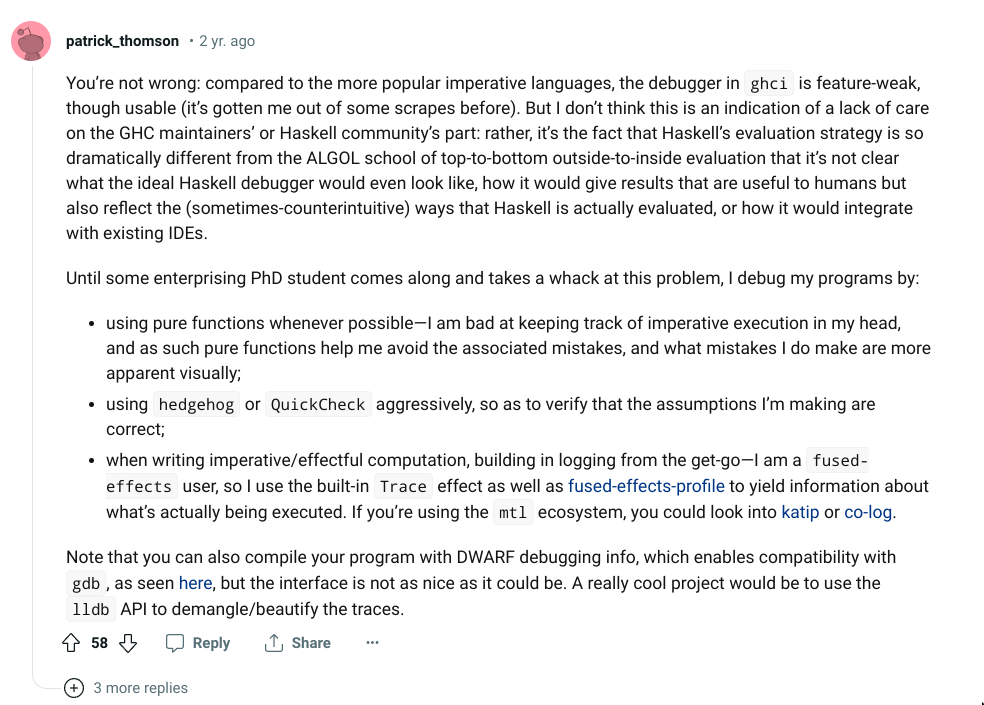
\includegraphics[width=\linewidth]{snapshots/haskell_debugging_is_hard01.png}
\end{frame}

\begin{frame}
	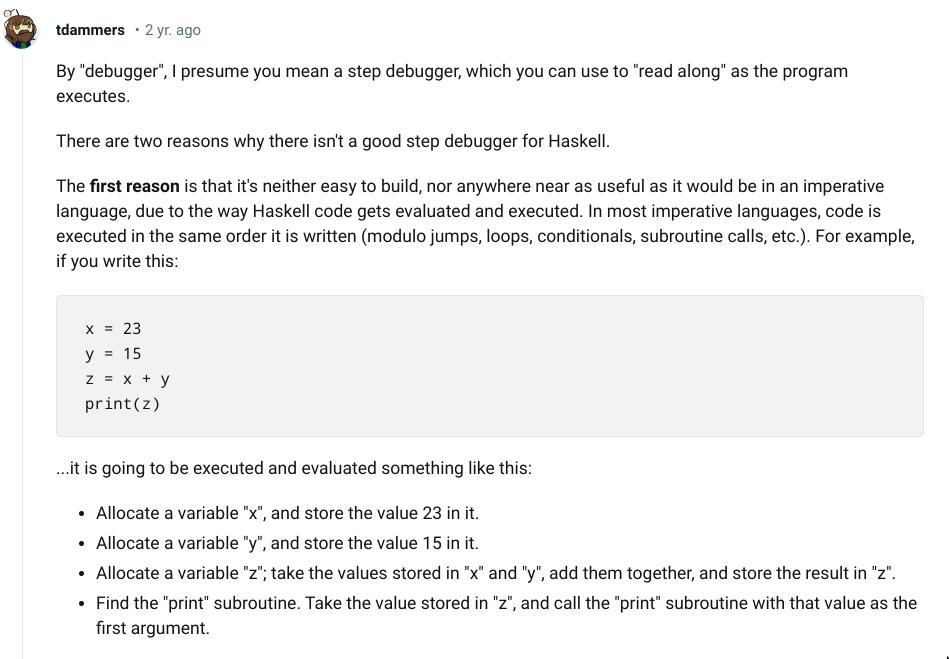
\includegraphics[width=\linewidth]{snapshots/haskell_debugging_is_hard02.png}
\end{frame}

\begin{frame}
	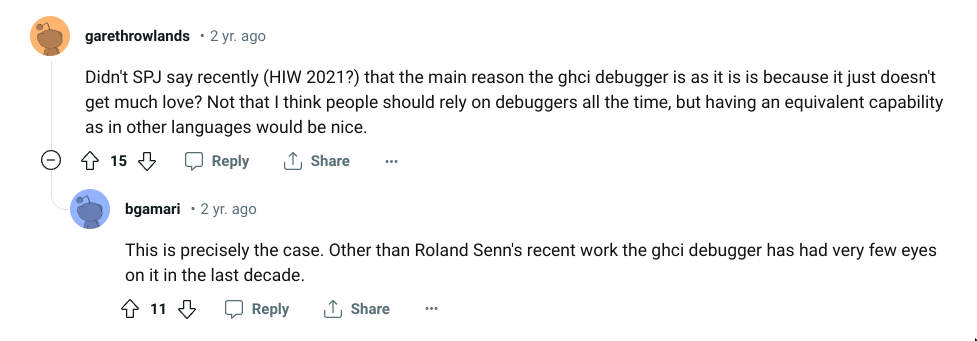
\includegraphics[width=\linewidth]{snapshots/haskell_debugging_is_hard03.png}
\end{frame}

\begin{frame}
\frametitle{Husky Debugging System: Expanding the computation graph into a Trace Tree}
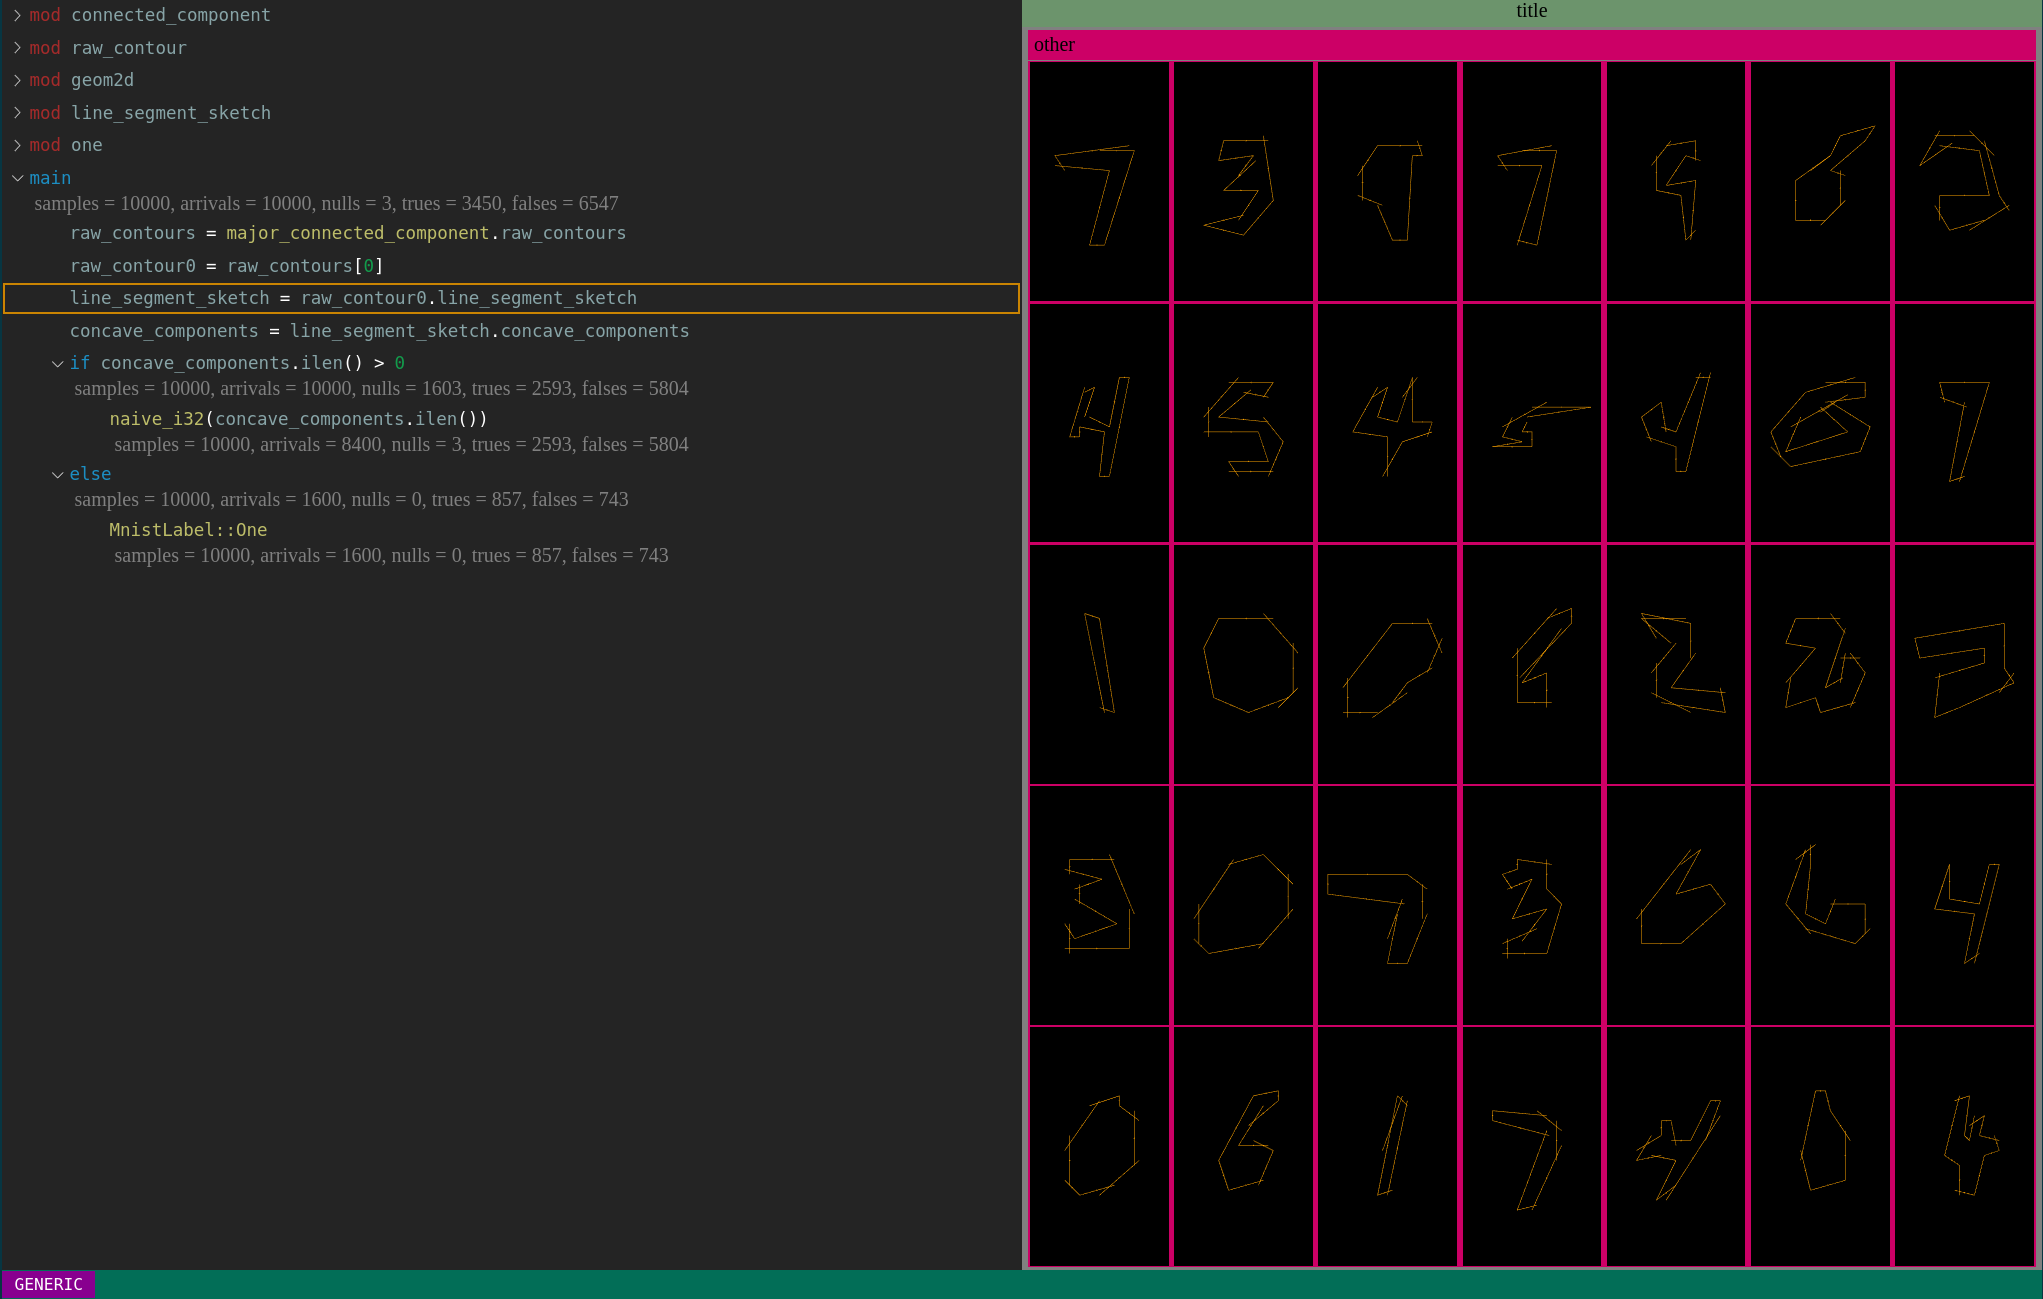
\includegraphics[width=\linewidth]{snapshots/trace-based-debugging-system.png}
\end{frame}
\end{document}